\part{模的演算}
\chapter{双侧纤维化与模}\label{ch:two-sided-fibrations-modules}


第 5 章中，我们研究过这样一些\trIsofibration：底范畴中的诸箭头以协变或逆变的
方式作用于其诸\trFiber。所谓\emph{\trCocartesianFibration}的一个原型例子，
是与\trArrowInfinityCategory{}相关联的余定义域投影\trFunctor{}
$p_{1}\colon A^{2}\twoheadrightarrow A$，其\trFiberwise{}作用由%
\trPostComposition{}给出；对偶地，定义域投影\trFunctor{}
$p_{0}\colon A^{2}\twoheadrightarrow A$ 是一条\trCartesianFibration，其%
\trFiberwise{}作用由\trPreComposition{}给出。本章中，我们通过把余定义域与定义域投影\trFunctor{}当作
一个\trSpan{} $A\xleftarrow{p_{1}}A^{2}\xrightarrow{p_{0}}A$（而非分而论之）
来考虑，精炼并加深对这些纤维化结构的理解。有几条观察旋即浮现。首先，%
$p_{1}$-余笛卡尔提升可以选取得定义一些以 $A^{2}$ 为余定义域的%
\trNaturalTransformation，其定义域分量皆为恒同；也就是说，$p_{1}$-余笛卡尔
提升可以选取得「位于 $p_{0}\colon A^{2}\twoheadrightarrow A$ 之上」。对偶地，
$p_{0}$-笛卡尔提升可以选取得位于 $p_{1}$ 之上（见命题 5.5.11）。

其次，\trFiberwise{}作用 $\alpha^{*}\colon\mathrm{Hom}_{A}(x,A)\to\mathrm{Hom}_{A}(w,A)$
——由余定义域为 $A$ 的\trNaturalTransformation{} $\alpha\colon w\Rightarrow x$
经\trPreComposition{}而得——在适当的意义下，与作用
$\gamma_{+}\colon\mathrm{Hom}_{A}(A,y)\to\mathrm{Hom}_{A}(A,z)$（由
$\gamma\colon y\Rightarrow z$ 经\trPostComposition{}而得）相交换。这前两条
性质概括起来就是说：与\trArrowInfinityCategory{}相关联的\trSpan{}定义了一个
从 $A$ 到 $A$ 的\emph{\trTwoSidedFibration}（two-sided fibration）。

最后，\trIsofibration{} $(p_{1},p_{0})\colon A^{2}\twoheadrightarrow A\times A$
的诸双纤维（bifibers）定义\trDiscrete{}\trInfinityCategory，即 $A$ 的诸%
\trMappingSpace。的确，当把 $A^{2}$ 视为 $A\times A$ 之上的%
\trSliceInfinityCosmos{}中的一个对象时，它本身就是\trDiscrete。这一附加性质
意味着：$A\xleftarrow{p_{1}}A^{2}\xrightarrow{p_{0}}A$ 定义一个从 $A$ 到 $A$
的\emph{\trDiscrete{}双侧纤维化}（discrete two-sided fibration），我们把它
简记作：$A^{2}$ 定义一个从 $A$ 到 $A$ 的\emph{\trModule}（module）。

回忆命题 6.3.14：对\trInfinityCosmos{} $\mathcal{K}$ 中任何\trInfinityCategory{}
$B$，以\trQuasiCategory{}富集的范畴 $\mathrm{co}\mathcal{C}\mathit{art}(\mathcal{K})_{/B}$
与 $\mathcal{C}\mathit{art}(\mathcal{K})_{/B}$ 都定义∞-宇宙，其\trLimit、%
\trIsofibration{}与\trEquivalence{}继承自它们向 $\mathcal{K}_{/B}$ 的%
\trCosmologicalEmbedding。本章中，我们将引入另一个\trCosmologicallyEmbedded{}∞-宇宙
${}_{A\backslash}\mathcal{F}\mathit{ib}(\mathcal{K})_{/B}\hookrightarrow\mathcal{K}_{/A\times B}$，
其对象是从 $A$ 到 $B$ 的\emph{\trTwoSidedFibration}（two-sided fibration）。
关于这一概念的若干\trEquivalence{}定义将在 7.1 节中给出。反复应用命题 6.3.14
即见 ${}_{A\backslash}\mathcal{F}\mathit{ib}(\mathcal{K})_{B}$ 仍是一个∞-宇宙，我们将在
7.2 节中研究它。

从 $B$ 到 $1$ 的\trTwoSidedFibration{}不过是 $B$ 上的一条%
\trCocartesianFibration，而从 $1$ 到 $B$ 的\trTwoSidedFibration{}则是
$B$ 上的一条\trCartesianFibration，因此关于\trTwoSidedFibration{}的诸结果
同时推广了这些单侧概念。7.2 节中发展的\trTwoSidedFibration{}的某些封闭性质
——例如对\trPullback{}的封闭——在第 5 章中已为读者所熟悉，而另一些，例如对%
\trSpan{}复合的封闭，则是双侧语境特有的。

在 7.3 节中，我们引入双侧可表示对象（two-sided representables），并证明%
\trYonedaLemma{}的一个双侧版本，将定理 5.7.3 与推论 5.7.19 加以推广。在%
\trYonedaLemma{}的诸种表述中，这是往后被证明最为有用的一种。

我们对\trTwoSidedFibration{}感兴趣的主要理由在于这样一个事实：%
${}_{A\backslash}\mathcal{F}\mathit{ib}(\mathcal{K})_{B}$ 中的\trDiscrete{}对象恰恰是
从 $A$ 到 $B$ 的\emph{\trModule}\footnote{在 1-范畴与∞-范畴的文献中，「分配子」
（distributor）[10]、「泛函子」（profunctor）[132]与「对应」（correspondence）
[5, 78]都被用作「模」的同义语。}，我们将在 7.4 节中定义并研究它们。第 8 章
发展的模的演算，是∞-范畴的形式范畴论的主要场所，而这正是第 9 章的主题。

\providecommand{\cellpair}[5]{$\vcenter{\hbox{\begin{tikzpicture}[x=1.15em,y=1.15em]%
\node (t) at (4.2,0) {$#2$};%
\draw[->] (0.75,0.32) to[bend left=18] (3.45,0.32);%
\node at (2.1,0.88) {$\scriptstyle#3$};%

\node at (2.1,0.88) {$\scriptstyle#3$};%
\draw[->] (0.75,-0.32) to[bend right=18] (3.45,-0.32);%
\node at (2.1,-0.93) {$\scriptstyle#4$};%
\draw[->] (1.95,0.2) to[bend right=32] (1.95,-0.2);%
\node at (2.85,0) {$\scriptstyle#5$};%
\end{tikzpicture}}}$\ignorespaces}

\section{双侧纤维化}\label{sec:two-sided-fibrations}

通过分解，∞-宇宙 $\mathcal{K}$ 中任何从 $A$ 到 $B$ 的\trSpan{}都可以在%
\trEquivalence{}意义下替换为一个\textbf{双侧\trIsofibration}（two-sided
isofibration），即一个跨度 $A\xleftarrow{q}E\xrightarrow{p}B$，使得\trFunctor{}
$(q,p)\colon E\twoheadrightarrow A\times B$ 是一条\trIsofibration{}。从 $A$ 到
$B$ 的\trTwoSidedIsofibration{}，正是 ∞-宇宙 $\mathcal{K}_{A\times B}$ 中的诸对象。在本节
中，我们描述一个\trTwoSidedIsofibration{}在何种意义上是\emph{左侧余笛卡尔的}或%
\emph{右侧笛卡尔的}，然后引入\emph{\trTwoSidedFibration}，它把这两种概念整合
起来。
为了给这些概念提供动机，考虑与 ∞-宇宙 $\mathcal{K}$ 中 $A$ 的%
\trArrowInfinityCategory{}相关联的跨度 $A\xleftarrow{p_{1}}A^{2}\xrightarrow{p_{0}}A$。在命题 5.5.11 中，我们观察到
\begin{center}
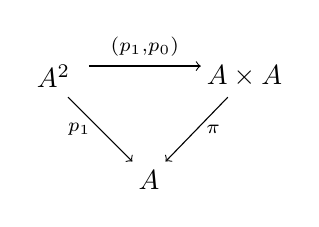
\begin{tikzpicture}[x=1.5em,y=1.5em]
  \node (A2) at (0,1.3) {$A^{2}$};
  \node (AA) at (4.6,1.3) {$A\times A$};
  \node (A)  at (2.3,-1.2) {$A$};
  \draw[->] (0.85,1.55) -- node[above]{$\scriptstyle(p_{1},p_{0})$} (3.55,1.55);
  \draw[->] (0.35,0.8) -- node[left,pos=0.5]{$\scriptstyle p_{1}$} (1.9,-0.75);
  \draw[->] (4.2,0.8) -- node[right,pos=0.5]{$\scriptstyle\pi$} (2.7,-0.75);
\end{tikzpicture}
\end{center}
定义了\trSliceInfinityCosmos{} $\mathcal{K}_{/A}$ 中的一条\trCartesianFibration%
——实际上是一条离散\trCartesianFibration{}，不过我们把对离散性的考量推迟到在
7.4 节中引入\emph{\trModule}之时。

该证明援引定理 5.2.8(iii)，它经由余定义域之上的一个\trFiberedAdjunction{}来刻画%
\trCartesianFibration{}。在此情形，该\trFiberedAdjunction{}位于 ∞-宇宙
$(\mathcal{K}_{/A})_{/\pi\colon A\times A\twoheadrightarrow A}\cong\mathcal{K}_{/A\times A}$ 之中，且等价于如下由诸指标范畴之间的一个伴随所产生的典范伴随
\begin{center}
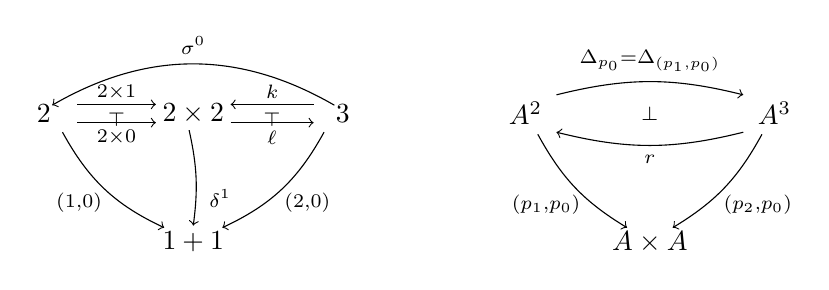
\begin{tikzpicture}[x=1.5em,y=1.5em]
  \node (two)  at (0,1.5) {$2$};
  \node (tt)   at (3.6,1.5) {$2\times 2$};
  \node (three) at (7.2,1.5) {$3$};
  \node (oo)   at (3.6,-1.6) {$1+1$};
  \draw[->] (7.0,1.7) to[bend right=30] node[above,pos=0.5]{$\scriptstyle\sigma^{0}$} (0.2,1.7);
  \draw[->] (0.8,1.72) -- (2.7,1.72);
  \node at (1.75,2.02) {$\scriptstyle 2\times 1$};
  \node at (1.75,1.36) {$\scriptstyle\top$};
  \draw[->] (0.8,1.28) -- (2.7,1.28);
  \node at (1.75,0.92) {$\scriptstyle 2\times 0$};
  \draw[->] (6.5,1.72) -- (4.5,1.72);
  \node at (5.5,2.02) {$\scriptstyle k$};
  \node at (5.5,1.36) {$\scriptstyle\top$};
  \draw[->] (4.5,1.28) -- (6.5,1.28);
  \node at (5.5,0.92) {$\scriptstyle\ell$};
  \draw[->] (0.45,1.05) to[bend right=18] (2.9,-1.25);
  \node at (0.85,-0.65) {$\scriptstyle(1,0)$};
  \draw[->] (6.75,1.05) to[bend left=18] (4.3,-1.25);
  \node at (6.35,-0.65) {$\scriptstyle(2,0)$};
  \draw[->] (3.5,1.1) to[bend left=10] (3.6,-1.2);
  \node at (4.25,-0.55) {$\scriptstyle\delta^{1}$};
  \node at (9.6,1.5) {$\twoheadrightarrow$};
  \begin{scope}[shift={(11.6,0)}]
  \node (A2)  at (0,1.5) {$A^{2}$};
  \node (A3)  at (6.0,1.5) {$A^{3}$};
  \node (AA)  at (3.0,-1.6) {$A\times A$};
  \draw[->] (0.75,1.95) to[bend left=14] node[above,pos=0.5]{$\scriptstyle\Delta_{p_{0}}=\Delta_{(p_{1},p_{0})}$} (5.25,1.95);
  \node at (3.0,1.5) {$\scriptstyle\perp$};
  \draw[->] (5.25,1.05) to[bend left=14] node[below,pos=0.5]{$\scriptstyle r$} (0.75,1.05);
  \draw[->] (0.3,1.0) to[bend right=15] (2.45,-1.25);
  \node at (0.5,-0.7) {$\scriptstyle(p_{1},p_{0})$};
  \draw[->] (5.7,1.0) to[bend left=15] (3.55,-1.25);
  \node at (5.6,-0.7) {$\scriptstyle(p_{2},p_{0})$};
  \end{scope}
\end{tikzpicture}
\end{center}
用我们即将引入的术语来说，这就是：\trTwoSidedIsofibration
$A\xleftarrow{p_{1}}A^{2}\xrightarrow{p_{0}}A$ 是\emph{右侧笛卡尔}的含义。

当我们与投向右因子的投影 $\pi\colon A\times A\twoheadrightarrow A$ 作%
\trPostComposition{}之后，便得到一个伴随
\begin{center}
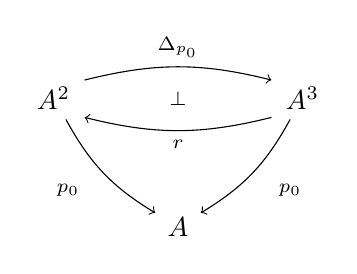
\begin{tikzpicture}[x=1.5em,y=1.5em]
  \node (A2) at (0,1.5) {$A^{2}$};
  \node (A3) at (6.0,1.5) {$A^{3}$};
  \node (A)  at (3.0,-1.6) {$A$};
  \draw[->] (0.75,1.95) to[bend left=14] node[above,pos=0.5]{$\scriptstyle\Delta_{p_{0}}$} (5.25,1.95);
  \node at (3.0,1.5) {$\scriptstyle\perp$};
  \draw[->] (5.25,1.05) to[bend left=14] node[below,pos=0.5]{$\scriptstyle r$} (0.75,1.05);
  \draw[->] (0.3,1.0) to[bend right=15] (2.45,-1.25);
  \node at (0.35,-0.7) {$\scriptstyle p_{0}$};
  \draw[->] (5.7,1.0) to[bend left=15] (3.55,-1.25);
  \node at (5.7,-0.7) {$\scriptstyle p_{0}$};
\end{tikzpicture}
\end{center}
它见证了命题 5.2.9 所确立的事实：$p_{0}\colon A^{2}\twoheadrightarrow A$ 是一条%
\trCartesianFibration{}。因此，说一个\trTwoSidedIsofibration{}是右侧笛卡尔的，其一部分含义
便是：它的右腿是一条\trCartesianFibration{}。说这个伴随位于 $A\times A$ 之上而不
仅仅位于 $A$ 之上，则等价于断言：$p_{0}$-笛卡尔提升可以选取得落在
$p_{1}\colon A^{2}\twoheadrightarrow A$ 的诸\trFiber{}之中，并且沿左腿须化后
成为恒同箭头。由此可知，每支 $p_{0}$-笛卡尔变换与 $p_{1}$ 须化后都是一个%
\trIsomorphism{}。

这两条性质还有另一种表达方式：即要求\trFunctor{}
\begin{center}
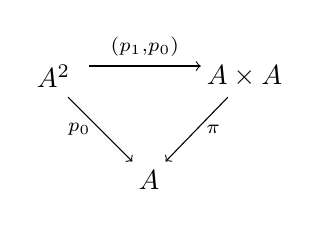
\begin{tikzpicture}[x=1.5em,y=1.5em]
  \node (A2) at (0,1.3) {$A^{2}$};
  \node (AA) at (4.6,1.3) {$A\times A$};
  \node (A)  at (2.3,-1.2) {$A$};
  \draw[->] (0.85,1.55) -- node[above]{$\scriptstyle(p_{1},p_{0})$} (3.55,1.55);
  \draw[->] (0.35,0.8) -- node[left,pos=0.5]{$\scriptstyle p_{0}$} (1.9,-0.75);
  \draw[->] (4.2,0.8) -- node[right,pos=0.5]{$\scriptstyle\pi$} (2.7,-0.75);
\end{tikzpicture}
\end{center}
落在 ∞-宇宙 $\mathcal{C}art(\mathcal{K})_{/A}\subset\mathcal{K}_{/A}$ 之中。
这首先断言 $p_{0}\colon A^{2}\twoheadrightarrow A$ 是一条\trCartesianFibration{}，
其次断言 $(p_{1},p_{0})$ 定义了从这个\trCartesianFibration{}到例 5.4.6 的%
\trCartesianFibration{} $\pi\colon A\times A\twoheadrightarrow A$ 的一个笛卡尔
函子。正如彼处所观察到的，诸 $\pi$-笛卡尔胞腔正是那些与另一个投影须化后成为%
\trIsomorphism{}的\trNaturalTransformation{}。于是，说 $(p_{1},p_{0})$ 是
一个\trCartesianFunctor{}，恰好就是说 $p_{1}$ 把诸 $p_{0}$-笛卡尔变换都送到\trIsomorphism{}。

我们现在把这些直觉形式化：

\begin{lemma}[右侧笛卡尔的]\label{lem:cartesian-on-the-right}
设 $A\xleftarrow{q}E\xrightarrow{p}B$ 是 ∞-宇宙 $\mathcal{K}$ 中的一个双侧等价
纤维化，则下列诸条等价：
\begin{enumerate}[label=(\roman*)]
\item \trFunctor{}
\begin{center}
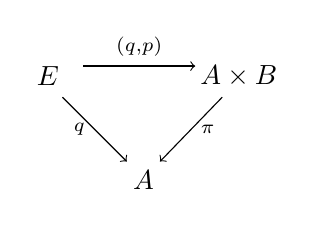
\begin{tikzpicture}[x=1.5em,y=1.5em]
  \node (E)  at (0,1.3) {$E$};
  \node (AB) at (4.6,1.3) {$A\times B$};
  \node (A)  at (2.3,-1.2) {$A$};
  \draw[->] (0.85,1.55) -- node[above]{$\scriptstyle(q,p)$} (3.55,1.55);
  \draw[->] (0.35,0.8) -- node[left,pos=0.5]{$\scriptstyle q$} (1.9,-0.75);
  \draw[->] (4.2,0.8) -- node[right,pos=0.5]{$\scriptstyle\pi$} (2.7,-0.75);
\end{tikzpicture}
\end{center}
是\trSliceInfinityCosmos{} $\mathcal{K}_{/A}$ 中的一条\trCartesianFibration{}。
\item \trFunctor{}
\begin{center}
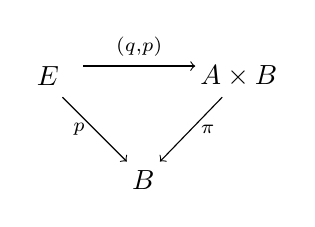
\begin{tikzpicture}[x=1.5em,y=1.5em]
  \node (E)  at (0,1.3) {$E$};
  \node (AB) at (4.6,1.3) {$A\times B$};
  \node (B)  at (2.3,-1.2) {$B$};
  \draw[->] (0.85,1.55) -- node[above]{$\scriptstyle(q,p)$} (3.55,1.55);
  \draw[->] (0.35,0.8) -- node[left,pos=0.5]{$\scriptstyle p$} (1.9,-0.75);
  \draw[->] (4.2,0.8) -- node[right,pos=0.5]{$\scriptstyle\pi$} (2.7,-0.75);
\end{tikzpicture}
\end{center}
在 $\mathcal{K}_{/B}$ 中落在子 ∞-宇宙 $\mathcal{C}art(\mathcal{K})_{/B}$ 之中。
\item 由 $\mathrm{id}_{p}$ 诱导的\trFunctor{}在 $\mathcal{K}_{/A\times B}$ 中
容有一个\trRightAdjoint{}：
\begin{center}
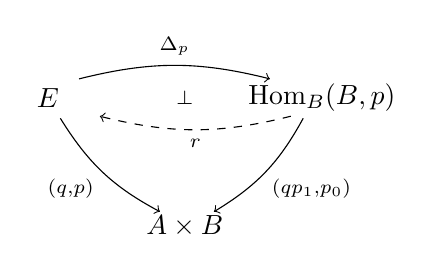
\begin{tikzpicture}[x=1.5em,y=1.5em]
  \node (E)   at (0,1.5) {$E$};
  \node (Hom) at (6.6,1.5) {$\mathrm{Hom}_{B}(B,p)$};
  \node (AB)  at (3.3,-1.6) {$A\times B$};
  \draw[->] (0.75,1.95) to[bend left=14] node[above,pos=0.5]{$\scriptstyle\Delta_{p}$} (5.35,1.95);
  \node at (3.3,1.5) {$\scriptstyle\perp$};
  \draw[->,dashed] (5.85,1.05) to[bend left=14] node[below,pos=0.5]{$\scriptstyle r$} (1.25,1.05);
  \draw[->] (0.3,1.0) to[bend right=15] (2.7,-1.25);
  \node at (0.55,-0.7) {$\scriptstyle(q,p)$};
  \draw[->] (6.15,1.0) to[bend left=15] (4.0,-1.25);
  \node at (6.35,-0.7) {$\scriptstyle(qp_{1},p_{0})$};
\end{tikzpicture}
\end{center}
\item 等价纤维化 $p\colon E\twoheadrightarrow B$ 是 $\mathcal{K}$ 中的一条%
\trCartesianFibration{}，并且对每支 $p$-笛卡尔变换
\cellpair{X}{E}{e'}{e}{\psi\psi}，其须化复合
\cellpair{X}{E}{e'}{e}{\psi\psi} $E\xrightarrow{q}A$
是一个\trIsomorphism{}。
\end{enumerate}
一个\trTwoSidedIsofibration $A\xleftarrow{q}E\xrightarrow{p}B$ 称为\textbf{右侧笛卡尔的}
（cartesian on the right），当这些等价条件被满足时。
\end{lemma}

\begin{proof}
等价 $(i)\Leftrightarrow(iii)$ 恰好是把定理 5.2.8(i)$\Leftrightarrow$(iii)
应用于\trSliceInfinityCosmos{} $\mathcal{K}_{/A}$ 中的等价纤维化
$(q,p)\colon E\twoheadrightarrow A\times B$ 而得的解读。后一结果断言：%
$\mathcal{K}_{/A}$ 中的等价纤维化 $(q,p)\colon E\twoheadrightarrow A\times B$
是一条\trCartesianFibration{}，当且仅当由 $\mathrm{id}_{(q,p)}$ 诱导的、从 $E$ 到%
\trFunctor{} $(q,p)\colon E\twoheadrightarrow A\times B$ 之右表示的那个%
\trFunctor{}容有一个余定义域 $\pi\colon A\times B\twoheadrightarrow A$ 之上的%
\trRightAdjoint{}；由于
$(\mathcal{K}_{/A})_{/\pi\colon A\times B\twoheadrightarrow A}\cong\mathcal{K}_{/A\times B}$，这与在 $A\times B$ 之上断言该伴随是一回事。

在 $\mathcal{K}_{/A}$ 中解读定理 5.2.8 的唯一微妙之处，在于为\trFunctor{}
$(q,p)\colon E\twoheadrightarrow A\times B$ 正确解读 $\mathcal{K}_{/A}$ 中的左
可表示\trCommaInfinityCategory{}。这个\trCommaInfinityCategory{}被构造为 $\mathcal{K}_{/A}$
中对象 $\pi\colon A\times B\to A$ 的 2-\trCotensor{}的一个\trSubobject{}，而命题
1.2.22 告诉我们，后者作为如下拉回方图的左侧竖直边而形成
\begin{center}
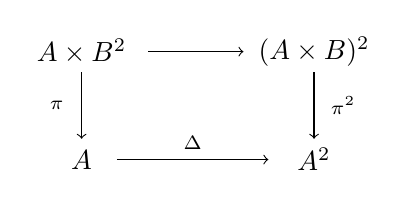
\begin{tikzpicture}[x=1.5em,y=1.5em]
  \node (AB2)  at (0,1.3) {$A\times B^{2}$};
  \node (AB2s) at (5.6,1.3) {$(A\times B)^{2}$};
  \node (A)    at (0,-1.3) {$A$};
  \node (A2)   at (5.6,-1.3) {$A^{2}$};
  \draw[->] (1.6,1.3) -- (3.9,1.3);
  \draw[->] (0,0.8) -- (0,-0.8);  \node at (-0.6,0) {$\scriptstyle\pi$};
  \draw[->] (5.6,0.8) -- (5.6,-0.8);  \node at (6.3,0) {$\scriptstyle\pi^{2}$};
  \draw[->] (0.85,-1.3) -- node[above]{$\scriptstyle\Delta$} (4.5,-1.3);
  \node at (0.55,0.75) {$\scriptstyle\llcorner$};
\end{tikzpicture}
\end{center}
按 (3.4.2)，这个\trCommaInfinityCategory{}由 $\mathcal{K}_{/A}$ 中的如下拉回
构造
\begin{rveq}\label{eq:slice-comma-pullback}
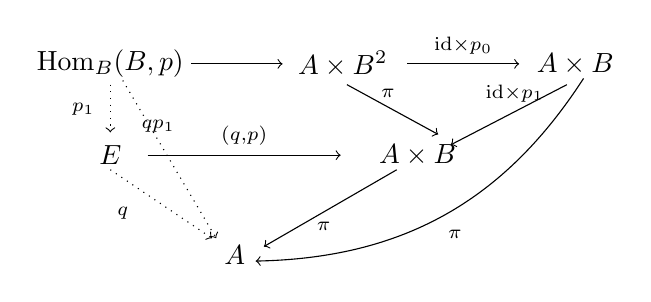
\begin{tikzpicture}[x=1.5em,y=1.5em]
  \node (Hom) at (0,2.6) {$\mathrm{Hom}_{B}(B,p)$};
  \node (AB2) at (5.6,2.6) {$A\times B^{2}$};
  \node (ABt) at (11.2,2.6) {$A\times B$};
  \node (E)   at (0,0.4) {$E$};
  \node (ABm) at (7.4,0.4) {$A\times B$};
  \node (A)   at (3.0,-2.0) {$A$};
  \draw[->] (1.95,2.6) -- (4.15,2.6);
  \draw[->] (7.15,2.6) -- node[above]{$\scriptstyle\mathrm{id}\times p_{0}$} (9.85,2.6);
  \draw[->,dotted] (0,2.1) -- (0,0.95);
  \node at (-0.65,1.5) {$\scriptstyle p_{1}$};
  \draw[->,dotted] (0.3,2.2) -- (2.55,-1.6);
  \node at (1.15,1.1) {$\scriptstyle qp_{1}$};
  \node at (0.55,2.3) {$\scriptstyle\lrcorner$};
  \draw[->] (5.7,2.1) -- node[above,pos=0.45]{$\scriptstyle\pi$} (7.9,0.9);
  \draw[->] (11.0,2.1) -- node[above,pos=0.45]{$\scriptstyle\mathrm{id}\times p_{1}$} (8.2,0.65);
  \draw[->] (0.9,0.4) -- node[above,pos=0.5]{$\scriptstyle(q,p)$} (5.55,0.4);
  \draw[->,dotted] (0,0.05) -- (2.45,-1.6);
  \node at (0.3,-1.0) {$\scriptstyle q$};
  \draw[->] (6.9,0.05) -- node[below,pos=0.55]{$\scriptstyle\pi$} (3.7,-1.8);
  \draw[->] (11.4,2.25) to[bend left=28] (3.5,-2.15);
  \node at (8.3,-1.5) {$\scriptstyle\pi$};
\end{tikzpicture}
\end{rveq}
该拉回由遗忘\trFunctor{} $\mathcal{K}_{/A}\to\mathcal{K}$ 所创造，且其余定义域
投影函子是顶部复合
$(qp_{1},p_{0})\colon\mathrm{Hom}_{B}(B,p)\twoheadrightarrow A\times B$。现在
我们看到，定理 5.2.8(i)$\Leftrightarrow$(iii) 在 $\mathcal{K}_{/A}$ 中的解读
恰好就是等价 $(i)\Leftrightarrow(iii)$。

剩下要论证的是与 (ii) 和 (iv) 的等价。假设 (iii) 并与
$\pi\colon A\times B\twoheadrightarrow B$ 复合，便得到一个\trFiberedAdjunction，后者证明
$p$ 是一条\trCartesianFibration{}。这两个\trFiberedAdjunction{}的\trCounit{}是同一个，并且由
定理 5.2.8(iii)，复合
\begin{center}
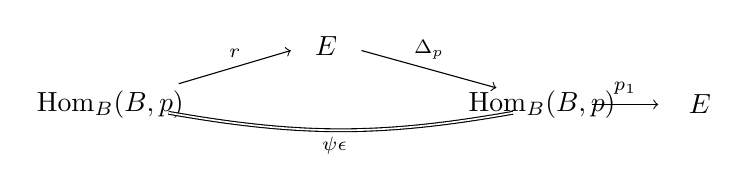
\begin{tikzpicture}[x=1.5em,y=1.5em]
  \node (H1) at (0,0) {$\mathrm{Hom}_{B}(B,p)$};
  \node (E)  at (5.2,1.4) {$E$};
  \node (H2) at (10.4,0) {$\mathrm{Hom}_{B}(B,p)$};
  \node (E2) at (14.2,0) {$E$};
  \draw[->] (1.65,0.5) -- node[above,pos=0.5]{$\scriptstyle r$} (4.35,1.3);
  \draw[->] (6.05,1.3) -- node[above,pos=0.5]{$\scriptstyle\Delta_{p}$} (9.3,0.4);
  \draw[double] (1.4,-0.2) to[bend right=10] (9.7,-0.2);
  \node at (5.4,-1.0) {$\scriptstyle\psi\epsilon$};
  \draw[->] (11.6,0) -- node[above,pos=0.5]{$\scriptstyle p_{1}$} (13.2,0);
\end{tikzpicture}
\end{center}
是泛 $p$-笛卡尔胞腔。由于 $\epsilon$ 在 $A\times B$ 之上纤维化，与 $q$ 作后
复合后便得到一个恒同，这就告诉我们 $q\colon E\twoheadrightarrow A$ 把诸 $p$-笛卡尔胞腔都送到%
\trIsomorphism{}。这证明了 (iii) 蕴涵 (iv)。

由例 5.4.6，\trCartesianFibration{} $\pi\colon A\times B\twoheadrightarrow B$
的诸笛卡尔胞腔恰好是那些余定义域为 $A$ 的分量为\trIsomorphism{}的 2-\trCell{}，
因此 (iv) 恰好说 $(q,p)\colon E\twoheadrightarrow A\times B$ 定义了从 $p$ 到
$\pi$ 的一个\trCartesianFunctor{}。于是 (iv) 蕴涵 (ii)。

为完成论证，我们来证明 (ii) 蕴涵 (i)。假设 (ii) 并考虑 $\mathcal{K}_{/A}$ 中的
一个 2-\trCell
\begin{center}
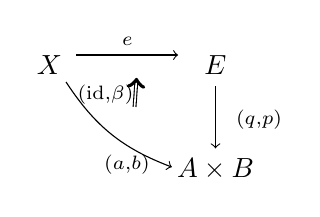
\begin{tikzpicture}[x=1.5em,y=1.5em]
  \node (X)  at (0,1.3) {$X$};
  \node (E)  at (4.0,1.3) {$E$};
  \node (AB) at (4.0,-1.2) {$A\times B$};
  \draw[->] (0.65,1.55) -- node[above]{$\scriptstyle e$} (3.1,1.55);
  \draw[->] (4.0,0.8) -- (4.0,-0.7);
  \node at (5.05,0) {$\scriptstyle(q,p)$};
  \draw[->] (0.4,0.9) to[bend right=18] node[below,pos=0.65]{$\scriptstyle(a,b)$} (2.95,-1.15);
  \draw[double,->] (2.05,0.3) -- (2.1,1.0);
  \node at (1.35,0.6) {$\scriptstyle(\mathrm{id},\beta)$};
\end{tikzpicture}
\end{center}
由于 $p$ 是一条\trCartesianFibration{}，$\beta\colon b\Rightarrow pe$ 容有一个
$p$-笛卡尔提升 $\chi\colon e'\Rightarrow e$；又由于 $(q,p)$ 是一个\trCartesianFunctor{}，
须化后的 2-\trCell{} $q\chi\colon qe'\Rightarrow a$ 是一个\trIsomorphism{}。由于
$(q,p)\colon E\twoheadrightarrow A\times B$ 是一条\trIsofibration{}，我们可以把
2-\trCell{} $(q\chi^{-1},\mathrm{id})\colon(a,b)\Rightarrow e'$ 提升为一个可逆
2-\trCell{} $\gamma\colon e''\Rightarrow e'$，满足 $p\gamma=\mathrm{id}_{b}$。
复合 $\chi\cdot\gamma\colon e''\Rightarrow e$ 是 $(\mathrm{id},\beta)$ 沿
$(q,p)$ 在 $A$ 之上的一个提升，且容易验证：它满足命题 5.2.11 所确立的、刻画
$\mathcal{K}_{/A}$ 中 $(\mathrm{id},\beta)$ 的 $(q,p)$-笛卡尔提升的那些弱%
\trUniversalProperty{}。这就证明了 (i)。
\end{proof}

合并\cref{lem:cartesian-on-the-right}及其对偶——后者定义了\textbf{左侧余笛卡尔的}
（cocartesian on the left）那类\trTwoSidedIsofibration——便得到：

\begin{corollary}\label{cor:cartesian-cocartesian-conditions}
∞-宇宙 $\mathcal{K}$ 中的一个\trTwoSidedIsofibration
$A\xleftarrow{q}E\xrightarrow{p}B$ 是左侧余笛卡尔的且是右侧笛卡尔的，若下列诸
等价条件被满足：
\begin{enumerate}[label=(\roman*)]
\item \trFunctor{}
\begin{center}
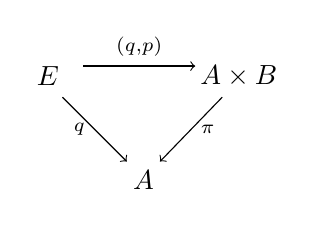
\begin{tikzpicture}[x=1.5em,y=1.5em]
  \node (E)  at (0,1.3) {$E$};
  \node (AB) at (4.6,1.3) {$A\times B$};
  \node (A)  at (2.3,-1.2) {$A$};
  \draw[->] (0.85,1.55) -- node[above]{$\scriptstyle(q,p)$} (3.55,1.55);
  \draw[->] (0.35,0.8) -- node[left,pos=0.5]{$\scriptstyle q$} (1.9,-0.75);
  \draw[->] (4.2,0.8) -- node[right,pos=0.5]{$\scriptstyle\pi$} (2.7,-0.75);
\end{tikzpicture}
\end{center}
落在 $\mathrm{co}\mathcal{C}\mathit{art}(\mathcal{K})_{/A}$ 之中，并定义 $\mathcal{K}_{/A}$
中的一条\trCartesianFibration{}。
\item \trFunctor{}
\begin{center}
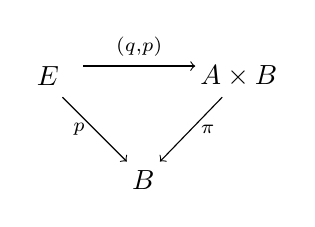
\begin{tikzpicture}[x=1.5em,y=1.5em]
  \node (E)  at (0,1.3) {$E$};
  \node (AB) at (4.6,1.3) {$A\times B$};
  \node (B)  at (2.3,-1.2) {$B$};
  \draw[->] (0.85,1.55) -- node[above]{$\scriptstyle(q,p)$} (3.55,1.55);
  \draw[->] (0.35,0.8) -- node[left,pos=0.5]{$\scriptstyle p$} (1.9,-0.75);
  \draw[->] (4.2,0.8) -- node[right,pos=0.5]{$\scriptstyle\pi$} (2.7,-0.75);
\end{tikzpicture}
\end{center}
落在 $\mathcal{C}art(\mathcal{K})_{/B}$ 之中，并定义 $\mathcal{K}_{/B}$ 中的一
条\trCocartesianFibration{}。
\end{enumerate}
\end{corollary}

一个\emph{\trTwoSidedFibration}是一个如下跨度：它左侧余笛卡尔、右侧笛卡尔，
并且满足一条进一步的相容性条件——该条件可以用若干种等价的方式来陈述，而这些
陈述归结为断言：取 $q$-余笛卡尔提升与取 $p$-笛卡尔提升这两个过程相互交换：

\begin{theorem}\label{thm:two-sided-fibration}
设 $A\xleftarrow{q}E\xrightarrow{p}B$ 是 ∞-宇宙 $\mathcal{K}$ 中的一个双侧等价
纤维化，则下列诸条等价：
\begin{enumerate}[label=(\roman*)]
\item \trFunctor{}
\begin{center}
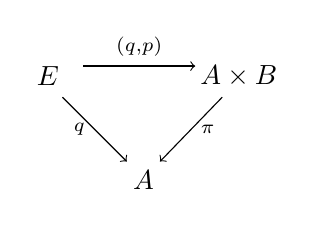
\begin{tikzpicture}[x=1.5em,y=1.5em]
  \node (E)  at (0,1.3) {$E$};
  \node (AB) at (4.6,1.3) {$A\times B$};
  \node (A)  at (2.3,-1.2) {$A$};
  \draw[->] (0.85,1.55) -- node[above]{$\scriptstyle(q,p)$} (3.55,1.55);
  \draw[->] (0.35,0.8) -- node[left,pos=0.5]{$\scriptstyle q$} (1.9,-0.75);
  \draw[->] (4.2,0.8) -- node[right,pos=0.5]{$\scriptstyle\pi$} (2.7,-0.75);
\end{tikzpicture}
\end{center}
定义了 $\mathrm{co}\mathcal{C}\mathit{art}(\mathcal{K})_{/A}$ 中的一条\trCartesianFibration{}。
\item \trFunctor{}
\begin{center}
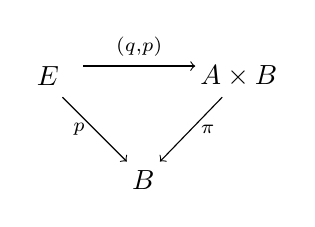
\begin{tikzpicture}[x=1.5em,y=1.5em]
  \node (E)  at (0,1.3) {$E$};
  \node (AB) at (4.6,1.3) {$A\times B$};
  \node (B)  at (2.3,-1.2) {$B$};
  \draw[->] (0.85,1.55) -- node[above]{$\scriptstyle(q,p)$} (3.55,1.55);
  \draw[->] (0.35,0.8) -- node[left,pos=0.5]{$\scriptstyle p$} (1.9,-0.75);
  \draw[->] (4.2,0.8) -- node[right,pos=0.5]{$\scriptstyle\pi$} (2.7,-0.75);
\end{tikzpicture}
\end{center}
定义了 $\mathcal{C}art(\mathcal{K})_{/B}$ 中的一条\trCocartesianFibration{}。
\item 诸典范\trFunctor{}在 $\mathcal{K}_{/A\times B}$ 中容有如下所示的诸伴随
\begin{center}
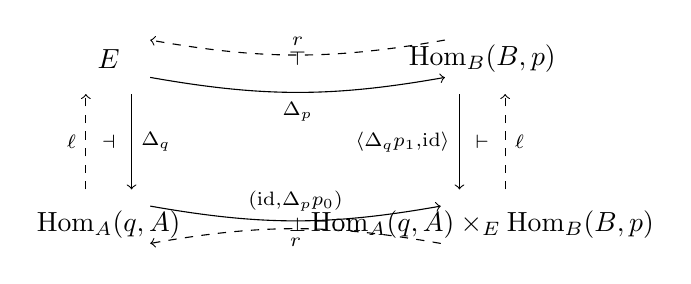
\begin{tikzpicture}[x=1.5em,y=1.5em]
  \node (E)    at (0,2.3) {$E$};
  \node (HomB) at (9.0,2.3) {$\mathrm{Hom}_{B}(B,p)$};
  \node (HomA) at (0,-1.7) {$\mathrm{Hom}_{A}(q,A)$};
  \node (P)    at (9.0,-1.7)
    {$\mathrm{Hom}_{A}(q,A)\times_{E}\mathrm{Hom}_{B}(B,p)$};
  \draw[->,dashed] (8.1,2.75) to[bend left=10] node[above,pos=0.5]{$\scriptstyle r$} (1.0,2.75);
  \node at (4.55,2.3) {$\scriptstyle\top$};
  \draw[->] (1.0,1.85) to[bend right=10] node[below,pos=0.5]{$\scriptstyle\Delta_{p}$} (8.1,1.85);
  \draw[->,dashed] (-0.55,-0.85) -- node[left,pos=0.5]{$\scriptstyle\ell$} (-0.55,1.45);
  \node at (0,0.3) {$\scriptstyle\dashv$};
  \draw[->] (0.55,1.45) -- node[right,pos=0.5]{$\scriptstyle\Delta_{q}$} (0.55,-0.85);
  \draw[->] (8.45,1.45) -- node[left,pos=0.5]{$\scriptstyle\langle\Delta_{q}p_{1},\mathrm{id}\rangle$} (8.45,-0.85);
  \node at (9.0,0.3) {$\scriptstyle\vdash$};
  \draw[->,dashed] (9.55,-0.85) -- node[right,pos=0.5]{$\scriptstyle\ell$} (9.55,1.45);
  \draw[->] (1.0,-1.25) to[bend right=10] node[above,pos=0.5]{$\scriptstyle(\mathrm{id},\Delta_{p}p_{0})$} (8.0,-1.25);
  \node at (4.55,-1.7) {$\scriptstyle\perp$};
  \draw[->,dashed] (8.0,-2.15) to[bend right=10] node[below,pos=0.5]{$\scriptstyle r$} (1.0,-2.15);
\end{tikzpicture}
\end{center}
并且该所示交换方块中恒同 2-胞腔的对应定义出一个同构 $\ell r\cong r\ell$。
\item \trTwoSidedIsofibration $A\xleftarrow{q}E\xrightarrow{p}B$ 是左侧余笛卡尔的、右侧
笛卡尔的，并且满足下述进一步的条件：给定如下左图所示的任一对%
\trNaturalTransformation{} $\alpha\colon qe\Rightarrow a$、
$\beta\colon b\Rightarrow pe$，以及如下右图所示的、$\alpha$ 在 $B$ 之上的
$q$-余笛卡尔提升 $\psi\colon e\Rightarrow\alpha_{*}e$ 与 $\beta$ 在 $A$ 之上的
$p$-笛卡尔提升 $\chi\colon\beta^{*}e\Rightarrow e$：
\begin{center}
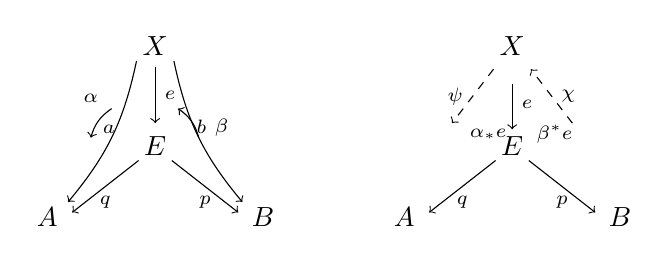
\begin{tikzpicture}[x=1.5em,y=1.5em]
  \begin{scope}[shift={(0,0)}]
  \node (X) at (2.6,1.5) {$X$};
  \node (E) at (2.6,-0.9) {$E$};
  \node (A) at (0,-2.6) {$A$};
  \node (B) at (5.2,-2.6) {$B$};
  \draw[->] (2.6,1.0) -- node[right,pos=0.5]{$\scriptstyle e$} (2.6,-0.35);
  \draw[->] (2.2,-1.25) -- node[below]{$\scriptstyle q$} (0.6,-2.5);
  \draw[->] (3.0,-1.25) -- node[below]{$\scriptstyle p$} (4.6,-2.5);
  \draw[->] (2.15,1.15) to[bend left=14] node[above,pos=0.55]{$\scriptstyle a$} (0.5,-2.25);
  \draw[->] (3.05,1.15) to[bend right=14] node[above,pos=0.55]{$\scriptstyle b$} (4.7,-2.25);
  \draw[->] (1.55,0.0) to[bend right=20] (1.05,-0.7);
  \node at (1.05,0.25) {$\scriptstyle\alpha$};
  \draw[->] (3.65,-0.7) to[bend right=20] (3.15,0.0);
  \node at (4.2,-0.45) {$\scriptstyle\beta$};
  \end{scope}
  \node at (7.3,-0.6) {$\twoheadrightarrow$};
  \begin{scope}[shift={(8.6,0)}]
  \node (X) at (2.6,1.5) {$X$};
  \node (E) at (2.6,-0.9) {$E$};
  \node (A) at (0,-2.6) {$A$};
  \node (B) at (5.2,-2.6) {$B$};
  \draw[->,dashed] (2.15,0.95) -- node[left,pos=0.5]{$\scriptstyle\psi$} (1.15,-0.35);
  \node at (2.02,-0.62) {$\scriptstyle\alpha_{*}e$};
  \draw[->] (2.6,0.6) -- node[right,pos=0.45]{$\scriptstyle e$} (2.6,-0.5);
  \draw[->,dashed] (4.05,-0.35) -- node[right,pos=0.5]{$\scriptstyle\chi$} (3.05,0.95);
  \node at (3.62,-0.62) {$\scriptstyle\beta^{*}e$};
  \draw[->] (2.2,-1.25) -- node[below]{$\scriptstyle q$} (0.6,-2.5);
  \draw[->] (3.0,-1.25) -- node[below]{$\scriptstyle p$} (4.6,-2.5);
  \end{scope}
\end{tikzpicture}
\end{center}
那么就存在一个在 $A\times B$ 之上的同构
$\alpha_{*}\beta^{*}e\cong\beta^{*}\alpha_{*}e$，它与 $\alpha\cdot q\chi$ 在
$B$ 之上的 $q$-余笛卡尔提升以及 $p\psi\cdot\beta$ 在 $A$ 之上的 $p$-笛卡尔提升
相交换：
\begin{center}
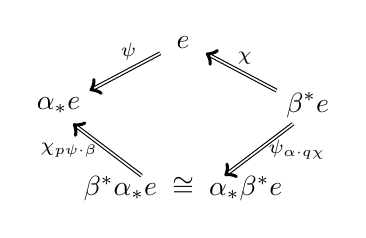
\begin{tikzpicture}[x=1.5em,y=1.5em]
  \node (e)    at (3.4,1.9) {$e$};
  \node (ase)  at (0.4,0.4) {$\alpha_{*}e$};
  \node (bse)  at (6.4,0.4) {$\beta^{*}e$};
  \node (bot)  at (3.4,-1.6) {$\beta^{*}\alpha_{*}e\;\cong\;\alpha_{*}\beta^{*}e$};
  \draw[double,->] (2.85,1.65) -- node[above,pos=0.45]{$\scriptstyle\psi$} (1.15,0.75);
  \draw[double,->] (5.65,0.75) -- node[above,pos=0.45]{$\scriptstyle\chi$} (3.95,1.65);
  \draw[double,->] (2.4,-1.3) -- node[left,pos=0.5]{$\scriptstyle\chi_{p\psi\cdot\beta}$} (0.75,-0.05);
  \draw[double,->] (6.05,-0.05) -- node[right,pos=0.5]{$\scriptstyle\psi_{\alpha\cdot q\chi}$} (4.4,-1.3);
\end{tikzpicture}
\end{center}
\end{enumerate}
当一个\trTwoSidedIsofibration $A\xleftarrow{q}E\xrightarrow{p}B$ 满足这些等价条件时，
它就定义了一个从 $A$ 到 $B$ 的\textbf{\trTwoSidedFibration}（two-sided
fibration）。
\end{theorem}

\begin{proof}
我们的策略是证明条件 (i) 等价于 (iii)——在切片 ∞-宇宙
$\mathcal{K}_{/A\times B}$ 中一个由等式见证的条件。对偶的论证表明条件 (ii)
等价于 (iii)。然后我们解析这个条件，以证明它与 (iv) 的等价。
若 (i) 成立，则 $A\xleftarrow{q}E\xrightarrow{p}B$ 也满足%
\cref{cor:cartesian-cocartesian-conditions}的条件 (i)，因为作为%
\trCartesianFibration{}这一性质被宇宙论\trFunctor{}
$\mathrm{co}\mathcal{C}\mathit{art}(\mathcal{K})_{/A}\hookrightarrow\mathcal{K}_{/A}$
所保持。于是 $A\xleftarrow{q}E\xrightarrow{p}B$ 特别地左侧余笛卡尔且右侧
笛卡尔，从而配备有伴随
\begin{center}
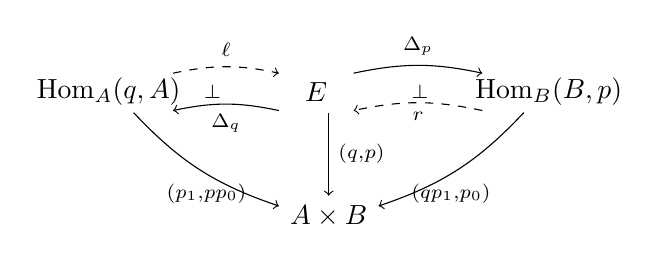
\begin{tikzpicture}[x=1.5em,y=1.5em]
  \node (HomA) at (0,1.5) {$\mathrm{Hom}_{A}(q,A)$};
  \node (E)    at (5.0,1.5) {$E$};
  \node (HomB) at (10.6,1.5) {$\mathrm{Hom}_{B}(B,p)$};
  \node (AB)   at (5.3,-1.5) {$A\times B$};
  \draw[->,dashed] (1.55,1.95) to[bend left=12] node[above,pos=0.5]{$\scriptstyle\ell$} (4.1,1.95);
  \node at (2.5,1.5) {$\scriptstyle\perp$};
  \draw[->] (4.1,1.05) to[bend right=12] node[below,pos=0.5]{$\scriptstyle\Delta_{q}$} (1.55,1.05);
  \draw[->] (5.9,1.95) to[bend left=12] node[above,pos=0.5]{$\scriptstyle\Delta_{p}$} (9.0,1.95);
  \node at (7.5,1.5) {$\scriptstyle\perp$};
  \draw[->,dashed] (9.0,1.05) to[bend right=12] node[below,pos=0.5]{$\scriptstyle r$} (5.9,1.05);
  \draw[->] (0.6,1.0) to[bend right=14] node[below,pos=0.55]{$\scriptstyle(p_{1},pp_{0})$} (4.1,-1.25);
  \draw[->] (5.3,1.0) -- node[right,pos=0.5]{$\scriptstyle(q,p)$} (5.3,-1.0);
  \draw[->] (10.0,1.0) to[bend left=14] node[below,pos=0.55]{$\scriptstyle(qp_{1},p_{0})$} (6.5,-1.25);
\end{tikzpicture}
\end{center}
由引理 3.6.6，我们可以把左手边的伴随沿
$A\times p_{1}\colon A\times B^{2}\twoheadrightarrow A\times B$ 拉回、再与
$A\times p_{0}\colon A\times B^{2}\twoheadrightarrow A\times B$ 复合，以得到下方右手边的%
\trFiberedAdjunction；并且同样把右手边的伴随沿
$p_{0}\times B\colon A^{2}\times B\twoheadrightarrow A\times B$ 拉回、再与
$p_{1}\times B\colon A^{2}\times B\twoheadrightarrow A\times B$ 复合，以得到下方左手边的%
\trFiberedAdjunction：
\begin{center}
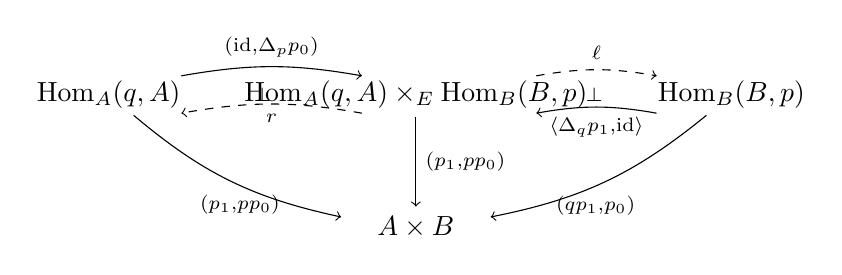
\begin{tikzpicture}[x=1.5em,y=1.5em]
  \node (HomA) at (0,1.5) {$\mathrm{Hom}_{A}(q,A)$};
  \node (P)    at (7.4,1.5)
    {$\mathrm{Hom}_{A}(q,A)\times_{E}\mathrm{Hom}_{B}(B,p)$};
  \node (HomB) at (15.0,1.5) {$\mathrm{Hom}_{B}(B,p)$};
  \node (AB)   at (7.4,-1.7) {$A\times B$};
  \draw[->] (1.75,1.95) to[bend left=10] node[above,pos=0.5]{$\scriptstyle(\mathrm{id},\Delta_{p}p_{0})$} (6.1,1.95);
  \node at (3.7,1.5) {$\scriptstyle\perp$};
  \draw[->,dashed] (6.1,1.05) to[bend right=10] node[below,pos=0.5]{$\scriptstyle r$} (1.75,1.05);
  \draw[->,dashed] (10.3,1.95) to[bend left=10] node[above,pos=0.5]{$\scriptstyle\ell$} (13.2,1.95);
  \node at (11.7,1.5) {$\scriptstyle\perp$};
  \draw[->] (13.2,1.05) to[bend right=10] node[below,pos=0.5]{$\scriptstyle\langle\Delta_{q}p_{1},\mathrm{id}\rangle$} (10.3,1.05);
  \draw[->] (7.4,0.95) -- node[right,pos=0.5]{$\scriptstyle(p_{1},pp_{0})$} (7.4,-1.2);
  \draw[->] (0.6,1.0) to[bend right=14] node[below,pos=0.55]{$\scriptstyle(p_{1},pp_{0})$} (5.6,-1.45);
  \draw[->] (14.4,1.0) to[bend left=14] node[below,pos=0.55]{$\scriptstyle(qp_{1},p_{0})$} (9.2,-1.45);
\end{tikzpicture}
\end{center}
尚待说明的是 (i) 中的假设——$(q,p)$ 定义
$\mathrm{co}\mathcal{C}\mathit{art}(\mathcal{K})_{/A}$ 中、而非仅仅 $\mathcal{K}_{/A}$
中的一条\trCartesianFibration{}。由定理 5.2.8(iii)，这个附加条件等价于断言：
右伴随
\begin{center}
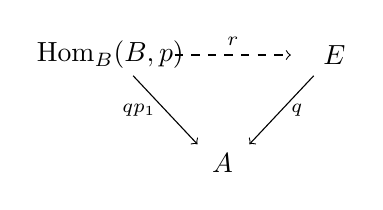
\begin{tikzpicture}[x=1.5em,y=1.5em]
  \node (Hom) at (0,1.3) {$\mathrm{Hom}_{B}(B,p)$};
  \node (E)   at (5.4,1.3) {$E$};
  \node (A)   at (2.7,-1.3) {$A$};
  \draw[->,dashed] (1.55,1.3) -- node[above]{$\scriptstyle r$} (4.35,1.3);
  \draw[->] (0.55,0.8) -- node[left,pos=0.5]{$\scriptstyle qp_{1}$} (2.1,-0.85);
  \draw[->] (4.9,0.8) -- node[right,pos=0.5]{$\scriptstyle q$} (3.35,-0.85);
\end{tikzpicture}
\end{center}
定义了从余笛卡尔纤维化 $p_{1}$ 到余笛卡尔纤维化 $q$ 的一个\trCartesianFunctor{}。由定理
5.3.4(iii)，这等价于断言：实线箭头方块
中同构的对应\footnote{实线箭头方块中的这个同构，是见证「$\Delta_{q}$ 定义了从
$p$ 到 $p_{0}$ 的一个\trCartesianFunctor」这一事实的那个对应的逆，而后者正是
$(q,p)$ 右侧笛卡尔的一部分含义。}
\begin{center}
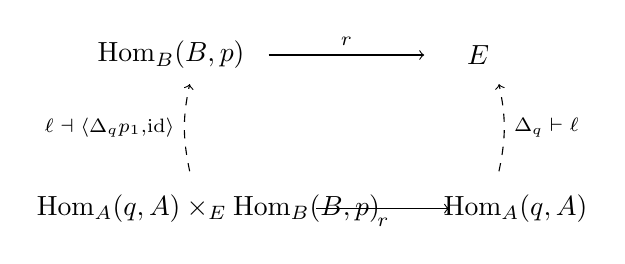
\begin{tikzpicture}[x=1.5em,y=1.5em]
  \node (Hom) at (0,2.2) {$\mathrm{Hom}_{B}(B,p)$};
  \node (E)   at (7.4,2.2) {$E$};
  \node (P)   at (0.9,-1.5)
    {$\mathrm{Hom}_{A}(q,A)\times_{E}\mathrm{Hom}_{B}(B,p)$};
  \node (HomA) at (8.3,-1.5) {$\mathrm{Hom}_{A}(q,A)$};
  \draw[->] (2.35,2.2) -- node[above]{$\scriptstyle r$} (6.1,2.2);
  \draw[->] (3.5,-1.5) -- node[below]{$\scriptstyle r$} (6.7,-1.5);
  \draw[->,dashed] (0.45,-0.6) to[bend left=12] node[left,pos=0.5]{$\scriptstyle\ell\;\dashv\;\langle\Delta_{q}p_{1},\mathrm{id}\rangle$} (0.45,1.5);
  \draw[->,dashed] (7.9,-0.6) to[bend right=12] node[right,pos=0.5]{$\scriptstyle\Delta_{q}\;\vdash\;\ell$} (7.9,1.5);
\end{tikzpicture}
\end{center}
定义了一个同构。这证明了 (i) 蕴涵 (iii)。

反之，假设 (iii)。由\cref{lem:cartesian-on-the-right}与%
\cref{cor:cartesian-cocartesian-conditions}，我们从其中两个伴随得出：%
\trFunctor{}
\begin{center}
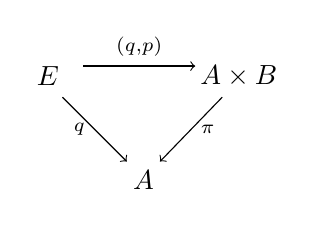
\begin{tikzpicture}[x=1.5em,y=1.5em]
  \node (E)  at (0,1.3) {$E$};
  \node (AB) at (4.6,1.3) {$A\times B$};
  \node (A)  at (2.3,-1.2) {$A$};
  \draw[->] (0.85,1.55) -- node[above]{$\scriptstyle(q,p)$} (3.55,1.55);
  \draw[->] (0.35,0.8) -- node[left,pos=0.5]{$\scriptstyle q$} (1.9,-0.75);
  \draw[->] (4.2,0.8) -- node[right,pos=0.5]{$\scriptstyle\pi$} (2.7,-0.75);
\end{tikzpicture}
\end{center}
\begingroup\emergencystretch=3em\sloppy
落在 $\mathrm{co}\mathcal{C}\mathit{art}(\mathcal{K})_{/A}$ 之中，并定义了
$\mathcal{K}_{/A}$ 里的一条\trCartesianFibration{}；
它也定义 $\mathrm{co}\mathcal{C}\mathit{art}(\mathcal{K})_{/A}$ 中的一条\trCartesianFibration，
当且仅当右伴随 $r$ 是从 $qp_{1}\colon\mathrm{Hom}_{B}(B,p)\twoheadrightarrow A$
到 $q\colon E\twoheadrightarrow A$
的一个\trCartesianFunctor{}（定理 5.2.8(iii)）；回忆包含
$\mathrm{co}\mathcal{C}\mathit{art}(\mathcal{K})_{/A}\hookrightarrow\mathcal{K}_{/A}$
在正维数箭头上是满的，因此在单位与余单位上没有可比较的条件。
由定理 5.3.4(iii)，这由对应 $\ell r\cong r\ell$ 的可逆性得出。
如此我们便看到 (iii) 蕴涵 (i)。
\endgroup

于是，我们已经证明：条件 (i) 等价于 (iii)——后者断言在 $\mathcal{K}_{/A\times B}$
中存在诸伴随，使得实线箭头图的所有对应都是同构。将这个论证对偶化，即可见 (iii)
等价于条件 (ii)。

最后，(iii) 与 (iv) 等价：因为 (iii) 中诸左伴随的存在性等价于该跨度左侧余
笛卡尔，诸右伴随的存在性等价于右侧笛卡尔，而笛卡尔提升与余笛卡尔提升的相容性
条件正是同构 $\ell r\cong r\ell$ 的含义。
\end{proof}

双侧纤维化的内部刻画有一个熟悉的推论：

\begin{corollary}\label{cor:two-sided-fibration-retract}
任何在 $A\times B$ 之上等价于某个\trTwoSidedFibration{}
$(q,p)\colon E\twoheadrightarrow A\times B$ 的\trTwoSidedIsofibration
$(a,b)\colon X\twoheadrightarrow A\times B$，都是一个\trTwoSidedFibration{}。
\end{corollary}

\begin{proof}
\cref{thm:two-sided-fibration}(iii) 的断言在\trFiberedEquivalence{}下不变。
\end{proof}

\cref{thm:two-sided-fibration}可用于确立一个涉及定义 1.1.4 之%
\trOrdinalCategory{}的重要例子族。

\begin{proposition}\label{prop:An-two-sided-fibration}
对任意\trInfinityCategory{} $A$ 与任意 $n\geq 2$，\trTwoSidedIsofibration
$A\xleftarrow{p_{n-1}}A^{n}\xrightarrow{p_{0}}A$ 定义了一个\trTwoSidedFibration{}。
\end{proposition}

这一结果是命题 5.5.11 及其对偶的推广，而其证明使用了类似的想法。

\begin{proof}
我们使用\cref{thm:two-sided-fibration}(iii)。与在\trInitial{}对象处的求值
$p_{0}\colon A^{\mathbb{n}}\to A$ 相关联的右表示\trCommaInfinityCategory{}由
如下拉回构造
\begin{center}
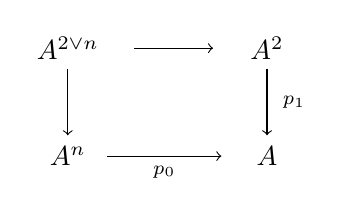
\begin{tikzpicture}[x=1.5em,y=1.5em]
  \node (A2vn) at (0,1.3) {$A^{2\vee\mathbb{n}}$};
  \node (A2)   at (4.8,1.3) {$A^{2}$};
  \node (An)   at (0,-1.3) {$A^{\mathbb{n}}$};
  \node (A)    at (4.8,-1.3) {$A$};
  \draw[->] (1.6,1.3) -- (3.5,1.3);
  \draw[->] (0,0.8) -- (0,-0.8);
  \node at (0.55,0.75) {$\scriptstyle\llcorner$};
  \draw[->] (4.8,0.8) -- (4.8,-0.8);
  \node at (5.45,0) {$\scriptstyle p_{1}$};
  \draw[->] (0.95,-1.3) -- node[below]{$\scriptstyle p_{0}$} (3.7,-1.3);
\end{tikzpicture}
\end{center}
它在诸\trEndpointEvaluation{}映射之下等价于
$(p_{n},p_{0})\colon A^{\mathbb{n}+\mathbb{1}}\twoheadrightarrow A\times A$。
检验 $(p_{n-1},p_{0})\colon A^{\mathbb{n}}\twoheadrightarrow A\times A$ 是否
右侧笛卡尔的典范\trFunctor{}，由沿\trEpimorphism{}
$\sigma^{0}\colon\mathbb{n}+\mathbb{1}\to\mathbb{n}$ 的限制给出，后者把
$\mathbb{n}+\mathbb{1}$ 中的对象 $0,1$ 送到 $\mathbb{n}$ 中的 $0$。该函子在诸%
\trEndpointInclusion{}之下容有一个左伴随
\begin{center}
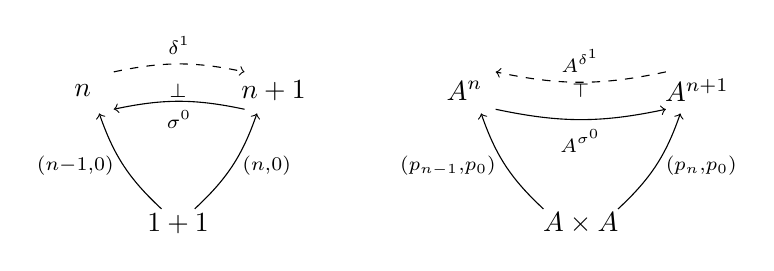
\begin{tikzpicture}[x=1.5em,y=1.5em]
  \node (n)  at (0,1.4) {$\mathbb{n}$};
  \node (n1) at (4.6,1.4) {$\mathbb{n}+\mathbb{1}$};
  \node (oo) at (2.3,-1.8) {$1+1$};
  \draw[->,dashed] (0.75,1.85) to[bend left=12] node[above,pos=0.5]{$\scriptstyle\delta^{1}$} (3.9,1.85);
  \node at (2.3,1.4) {$\scriptstyle\perp$};
  \draw[->] (3.9,0.95) to[bend right=12] node[below,pos=0.5]{$\scriptstyle\sigma^{0}$} (0.75,0.95);
  \draw[->] (1.9,-1.45) to[bend left=14] node[left,pos=0.5]{$\scriptstyle(n-1,0)$} (0.4,0.85);
  \draw[->] (2.7,-1.45) to[bend right=14] node[right,pos=0.5]{$\scriptstyle(n,0)$} (4.2,0.85);
  \node at (7.0,1.4) {$\twoheadrightarrow$};
  \begin{scope}[shift={(9.2,0)}]
  \node (An)  at (0,1.4) {$A^{\mathbb{n}}$};
  \node (An1) at (5.6,1.4) {$A^{\mathbb{n}+\mathbb{1}}$};
  \node (AA)  at (2.8,-1.8) {$A\times A$};
  \draw[->,dashed] (4.85,1.85) to[bend left=12] node[above,pos=0.5]{$\scriptstyle A^{\delta^{1}}$} (0.75,1.85);
  \node at (2.8,1.4) {$\scriptstyle\top$};
  \draw[->] (0.75,0.95) to[bend right=12] node[below,pos=0.5]{$\scriptstyle A^{\sigma^{0}}$} (4.85,0.95);
  \draw[->] (1.9,-1.45) to[bend left=14] node[left,pos=0.5]{$\scriptstyle(p_{n-1},p_{0})$} (0.4,0.85);
  \draw[->] (3.7,-1.45) to[bend right=14] node[right,pos=0.5]{$\scriptstyle(p_{n},p_{0})$} (5.2,0.85);
  \end{scope}
\end{tikzpicture}
\end{center}
如此便给出了上方左图所示的所求纤维化右伴随。

对偶的论证表明 $(p_{n-1},p_{0})\colon A^{\mathbb{n}}\twoheadrightarrow A\times A$ 是左侧余笛卡尔的。最后的条件要求：由诸\trDegeneracyOperator{}定义的交换方块的对应
\begin{center}
\begin{tikzpicture}[x=1.5em,y=1.5em]
  \node (n)   at (0,2.2) {$\mathbb{n}$};
  \node (n1t) at (4.6,2.2) {$\mathbb{n}+\mathbb{1}$};
  \node (n1b) at (0,-1.6) {$\mathbb{n}+\mathbb{1}$};
  \node (n2)  at (4.6,-1.6) {$\mathbb{n}+2$};
  \draw[->,dashed] (0.75,2.65) to[bend left=12] node[above,pos=0.5]{$\scriptstyle\delta^{1}$} (3.9,2.65);
  \node at (2.3,2.2) {$\scriptstyle\perp$};
  \draw[->] (3.9,1.75) to[bend right=12] node[below,pos=0.5]{$\scriptstyle\sigma^{0}$} (0.75,1.75);
  \draw[->] (3.9,-1.15) to[bend right=12] node[above,pos=0.5]{$\scriptstyle\sigma^{0}$} (0.75,-1.15);
  \node at (2.3,-1.6) {$\scriptstyle\top$};
  \draw[->,dashed] (0.75,-2.05) to[bend left=12] node[below,pos=0.5]{$\scriptstyle\delta^{1}$} (3.9,-2.05);
  \draw[->,dashed] (-0.55,1.45) to[bend left=14] node[left,pos=0.5]{$\scriptstyle\delta^{n}\;\dashv\;\sigma^{n}$} (-0.55,0.15);
  \draw[->,dashed] (5.15,0.15) to[bend left=14] node[right,pos=0.5]{$\scriptstyle\sigma^{n+1}\;\dashv\;\delta^{n+1}$} (5.15,1.45);
\end{tikzpicture}
\end{center}
是同构，编码了诸单纯恒等式中我们熟悉的一个。\cref{thm:two-sided-fibration}(iii)%
中的方块可通过应用 $A^{(-)}$ 而得到。
\end{proof}

我们把对双侧纤维化这一类对象的诸封闭性质的进一步讨论推迟到下一节，在那里我们
将部署宇宙论的论证来精简它们的证明。这些观察使我们得以进一步扩充我们的例子族。

为那一工作做准备，我们考虑双侧纤维化之间的保结构态射，证明%
\cref{thm:two-sided-fibration}的一个相对类比：

\begin{proposition}\label{prop:map-of-spans}
对于 ∞-宇宙 $\mathcal{K}$ 中一对从 $A$ 到 $B$ 的双侧纤维化之间的如下跨度映射
\begin{center}
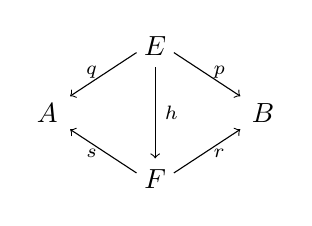
\begin{tikzpicture}[x=1.5em,y=1.5em]
  \node (E) at (2.6,1.6) {$E$};
  \node (A) at (0,0) {$A$};
  \node (B) at (5.2,0) {$B$};
  \node (F) at (2.6,-1.6) {$F$};
  \draw[->] (2.15,1.45) -- node[above,left,pos=0.45]{$\scriptstyle q$} (0.55,0.4);
  \draw[->] (3.05,1.45) -- node[above,right,pos=0.45]{$\scriptstyle p$} (4.65,0.4);
  \draw[->] (2.6,1.1) -- node[right,pos=0.5]{$\scriptstyle h$} (2.6,-1.1);
  \draw[->] (2.15,-1.45) -- node[below,left,pos=0.45]{$\scriptstyle s$} (0.55,-0.4);
  \draw[->] (3.05,-1.45) -- node[below,right,pos=0.45]{$\scriptstyle r$} (4.65,-0.4);
\end{tikzpicture}
\end{center}
下列诸条等价：
\begin{enumerate}[label=(\roman*)]
\item $h$ 定义了 $\mathrm{co}\mathcal{C}\mathit{art}(\mathcal{K})_{/A}$ 中诸%
\trCartesianFibration{}之间的一个\trCartesianFunctor{}。
\item $h$ 定义了 $\mathcal{C}art(\mathcal{K})_{/B}$ 中诸%
\trCocartesianFibration{}之间的一个\trCartesianFunctor{}。
\item 诸典范同构
\begin{center}
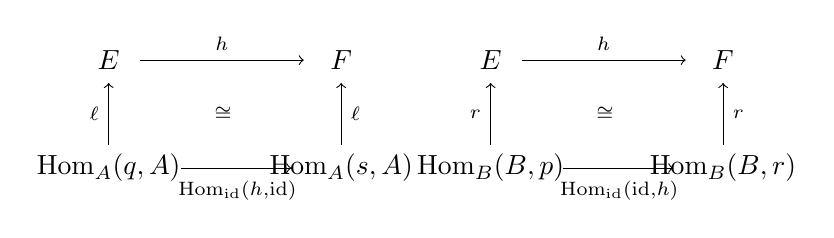
\begin{tikzpicture}[x=1.5em,y=1.5em]
  \node (E1) at (0,1.3) {$E$};
  \node (F1) at (5.6,1.3) {$F$};
  \node (H1) at (0,-1.3) {$\mathrm{Hom}_{A}(q,A)$};
  \node (H2) at (5.6,-1.3) {$\mathrm{Hom}_{A}(s,A)$};
  \draw[->] (0.75,1.3) -- node[above]{$\scriptstyle h$} (4.7,1.3);
  \draw[->] (0,-0.75) -- node[left]{$\scriptstyle\ell$} (0,0.75);
  \draw[->] (5.6,-0.75) -- node[right]{$\scriptstyle\ell$} (5.6,0.75);
  \draw[->] (1.75,-1.3) -- (4.4,-1.3);
  \node at (3.1,-1.85) {$\scriptstyle\mathrm{Hom}_{\mathrm{id}}(h,\mathrm{id})$};
  \node at (2.8,0) {$\scriptstyle\cong\,\curvearrowleft$};
  \begin{scope}[shift={(9.2,0)}]
  \node (E2) at (0,1.3) {$E$};
  \node (F2) at (5.6,1.3) {$F$};
  \node (H3) at (0,-1.3) {$\mathrm{Hom}_{B}(B,p)$};
  \node (H4) at (5.6,-1.3) {$\mathrm{Hom}_{B}(B,r)$};
  \draw[->] (0.75,1.3) -- node[above]{$\scriptstyle h$} (4.7,1.3);
  \draw[->] (0,-0.75) -- node[left]{$\scriptstyle r$} (0,0.75);
  \draw[->] (5.6,-0.75) -- node[right]{$\scriptstyle r$} (5.6,0.75);
  \draw[->] (1.75,-1.3) -- (4.4,-1.3);
  \node at (3.1,-1.85) {$\scriptstyle\mathrm{Hom}_{\mathrm{id}}(\mathrm{id},h)$};
  \node at (2.8,0) {$\scriptstyle\cong\,\curvearrowleft$};
  \end{scope}
\end{tikzpicture}
\end{center}
的对应定义了 $\mathcal{K}_{/A\times B}$ 中的同构。
\item 在 $\mathcal{K}$ 中，$h$ 定义了余笛卡尔纤维化 $q$ 与 $s$ 之间的一个笛卡尔
函子，以及笛卡尔纤维化 $p$ 与 $r$ 之间的一个\trCartesianFunctor{}。
\end{enumerate}
当这些等价条件被满足时，该跨度映射就定义了从 $A$ 到 $B$ 的双侧纤维化之间的一个%
\textbf{\trCartesianFunctor}（cartesian functor）。
\end{proposition}

\begin{proof}
由定理 5.3.4(iii)，条件 (iv) 等价于要求 (iii) 中所示的两个对应分别是
$\mathcal{K}_{/A}$ 与 $\mathcal{K}_{/B}$ 中的同构。但由于这些跨度是从 $A$ 到
$B$ 的双侧纤维化，且 $h$ 是 $A\times B$ 之上的映射，这两个%
\trNaturalTransformation{}都位于 $\mathcal{K}_{/A\times B}$ 之中。由命题
3.6.2，如果这些\trNaturalTransformation{}在 $\mathcal{K}_{/A}$ 与
$\mathcal{K}_{/B}$ 中容有逆，那么这些逆变换就提升为 $\mathcal{K}_{/A\times B}$
中的一个逆同构。这证明了 (iv) 等价于 (iii)。

我们接下来证明 (i) 等价于 (iii)。(ii) 与 (iii) 之等价的证明是对偶的。要像
(i) 中那样断言映射
\begin{center}
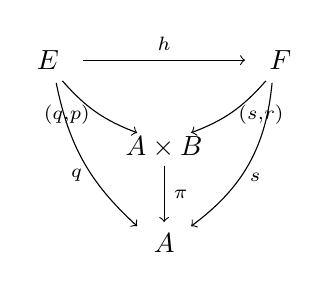
\begin{tikzpicture}[x=1.5em,y=1.5em]
  \node (E)  at (0,2.4) {$E$};
  \node (F)  at (5.6,2.4) {$F$};
  \node (AB) at (2.8,0.3) {$A\times B$};
  \node (A)  at (2.8,-2.0) {$A$};
  \draw[->] (0.85,2.4) -- node[above]{$\scriptstyle h$} (4.75,2.4);
  \draw[->] (0.35,1.9) to[bend right=14] node[left,pos=0.55]{$\scriptstyle(q,p)$} (2.15,0.65);
  \draw[->] (5.25,1.9) to[bend left=14] node[right,pos=0.55]{$\scriptstyle(s,r)$} (3.45,0.65);
  \draw[->] (0.2,1.85) to[bend right=18] node[left,pos=0.6]{$\scriptstyle q$} (2.15,-1.6);
  \draw[->] (5.4,1.85) to[bend left=24] node[right,pos=0.6]{$\scriptstyle s$} (3.45,-1.6);
  \draw[->] (2.8,-0.15) -- node[right,pos=0.5]{$\scriptstyle\pi$} (2.8,-1.5);
\end{tikzpicture}
\end{center}
定义了 $\mathrm{co}\mathcal{C}\mathit{art}(\mathcal{K})_{/A}$ 中诸%
\trCartesianFibration{}之间的一个\trCartesianFunctor{}，首先意味着对应
\begin{center}
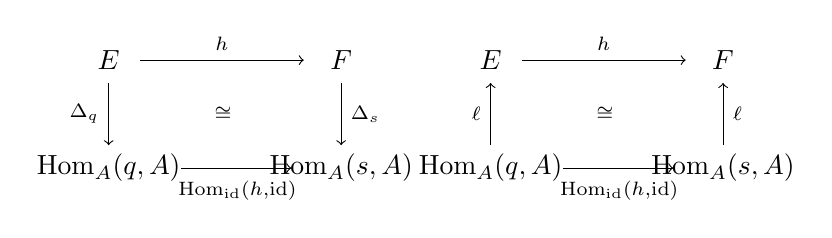
\begin{tikzpicture}[x=1.5em,y=1.5em]
  \node (E1) at (0,1.3) {$E$};
  \node (F1) at (5.6,1.3) {$F$};
  \node (H1) at (0,-1.3) {$\mathrm{Hom}_{A}(q,A)$};
  \node (H2) at (5.6,-1.3) {$\mathrm{Hom}_{A}(s,A)$};
  \draw[->] (0.75,1.3) -- node[above]{$\scriptstyle h$} (4.7,1.3);
  \draw[->] (0,0.75) -- node[left]{$\scriptstyle\Delta_{q}$} (0,-0.75);
  \draw[->] (5.6,0.75) -- node[right]{$\scriptstyle\Delta_{s}$} (5.6,-0.75);
  \draw[->] (1.75,-1.3) -- (4.4,-1.3);
  \node at (3.1,-1.85) {$\scriptstyle\mathrm{Hom}_{\mathrm{id}}(h,\mathrm{id})$};
  \node at (2.8,0) {$\scriptstyle\cong\,\curvearrowleft$};
  \node at (7.6,0) {$\rightsquigarrow$};
  \begin{scope}[shift={(9.2,0)}]
  \node (E2) at (0,1.3) {$E$};
  \node (F2) at (5.6,1.3) {$F$};
  \node (H3) at (0,-1.3) {$\mathrm{Hom}_{A}(q,A)$};
  \node (H4) at (5.6,-1.3) {$\mathrm{Hom}_{A}(s,A)$};
  \draw[->] (0.75,1.3) -- node[above]{$\scriptstyle h$} (4.7,1.3);
  \draw[->] (0,-0.75) -- node[left]{$\scriptstyle\ell$} (0,0.75);
  \draw[->] (5.6,-0.75) -- node[right]{$\scriptstyle\ell$} (5.6,0.75);
  \draw[->] (1.75,-1.3) -- (4.4,-1.3);
  \node at (3.1,-1.85) {$\scriptstyle\mathrm{Hom}_{\mathrm{id}}(h,\mathrm{id})$};
  \node at (2.8,0) {$\scriptstyle\cong\,\curvearrowleft$};
  \end{scope}
\end{tikzpicture}
\end{center}
定义了 $\mathcal{K}_{/A}$ 中的一个同构——因为 $h$ 在 $A$ 之上定义了余笛卡尔
纤维化 $q$ 与 $s$ 之间的一个\trCartesianFunctor{}；其次意味着对应
\begin{center}
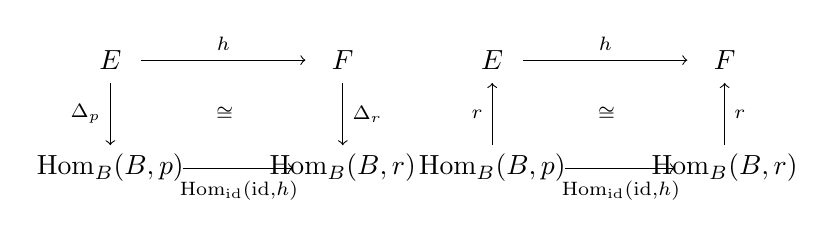
\begin{tikzpicture}[x=1.5em,y=1.5em]
  \node (E1) at (0,1.3) {$E$};
  \node (F1) at (5.6,1.3) {$F$};
  \node (H1) at (0,-1.3) {$\mathrm{Hom}_{B}(B,p)$};
  \node (H2) at (5.6,-1.3) {$\mathrm{Hom}_{B}(B,r)$};
  \draw[->] (0.75,1.3) -- node[above]{$\scriptstyle h$} (4.7,1.3);
  \draw[->] (0,0.75) -- node[left]{$\scriptstyle\Delta_{p}$} (0,-0.75);
  \draw[->] (5.6,0.75) -- node[right]{$\scriptstyle\Delta_{r}$} (5.6,-0.75);
  \draw[->] (1.75,-1.3) -- (4.4,-1.3);
  \node at (3.1,-1.85) {$\scriptstyle\mathrm{Hom}_{\mathrm{id}}(\mathrm{id},h)$};
  \node at (2.8,0) {$\scriptstyle\cong\,\curvearrowleft$};
  \node at (7.6,0) {$\rightsquigarrow$};
  \begin{scope}[shift={(9.2,0)}]
  \node (E2) at (0,1.3) {$E$};
  \node (F2) at (5.6,1.3) {$F$};
  \node (H3) at (0,-1.3) {$\mathrm{Hom}_{B}(B,p)$};
  \node (H4) at (5.6,-1.3) {$\mathrm{Hom}_{B}(B,r)$};
  \draw[->] (0.75,1.3) -- node[above]{$\scriptstyle h$} (4.7,1.3);
  \draw[->] (0,-0.75) -- node[left]{$\scriptstyle r$} (0,0.75);
  \draw[->] (5.6,-0.75) -- node[right]{$\scriptstyle r$} (5.6,0.75);
  \draw[->] (1.75,-1.3) -- (4.4,-1.3);
  \node at (3.1,-1.85) {$\scriptstyle\mathrm{Hom}_{\mathrm{id}}(\mathrm{id},h)$};
  \node at (2.8,0) {$\scriptstyle\cong\,\curvearrowleft$};
  \end{scope}
\end{tikzpicture}
\end{center}
是 $(\mathrm{co}\mathcal{C}\mathit{art}(\mathcal{K})_{/A})_{/\pi}$ 中的一个同构。由于
这些跨度是双侧纤维化，且 $h$ 是 $A\times B$ 之上的映射，第一对对应位于
$\mathcal{K}_{/A\times B}$ 之中。而由于包含
$(\mathrm{co}\mathcal{C}\mathit{art}(\mathcal{K})_{/A})_{/\pi}\hookrightarrow\mathcal{K}_{/A\times B}$ 在正维数箭头上是满的，要求第二对对应是
$(\mathrm{co}\mathcal{C}\mathit{art}(\mathcal{K})_{/A})_{/\pi}$ 中的同构，就等价于要求
同一条件在 $\mathcal{K}_{/A\times B}$ 中成立。这就证明了与 (iii) 的等价。
\end{proof}


这由\cref{thm:two-sided-fibration}与\cref{prop:map-of-spans}的内部刻画可得。

\begin{corollary}\label{cor:cosmological-preserves-two-sided}
任何宇宙论\trFunctor{}都保持\trTwoSidedFibration{}以及它们之间的\trCartesianFunctor{}。
\end{corollary}

\begin{proof}
由命题 1.3.4(vi)，任何宇宙论\trFunctor{} $F\colon\mathcal{K}\to\mathcal{L}$
对 $\mathcal{K}$ 中任意一对\trInfinityCategory{} $A$ 与 $B$ 都诱导一个宇宙论%
\trFunctor{} $F'\colon\mathcal{K}_{/A\times B}\to\mathcal{L}_{/FA\times FB}$。
该\trFunctor{}保持\cref{thm:two-sided-fibration}(iii) 的诸\trFiberedAdjunction{}与可逆
对应。于是
$F\colon\mathcal{K}\to\mathcal{L}$ 保持双侧纤维化；类似地，任何宇宙论%
\trFunctor{}都保持\cref{prop:map-of-spans}(iii) 的可逆对应。
\end{proof}


\subsection*{练习}

\begin{exercise}\label{ex:product-projection-span}
证明：对任意\trInfinityCategory{} $A$ 与 $B$，乘积投影跨度
$A\xleftarrow{\pi}A\times B\xrightarrow{\pi}B$ 定义了一个\trTwoSidedFibration{}。
\end{exercise}

\begin{exercise}\label{ex:two-sided-from-terminal}
证明：
\begin{enumerate}[label=(\roman*)]
\item \trTwoSidedIsofibration $1\xleftarrow{!}E\xrightarrow{p}B$ 定义了从 $1$ 到 $B$
的一个\trTwoSidedFibration{}，当且仅当 $p\colon E\twoheadrightarrow B$ 是一条%
\trCartesianFibration{}。
\item 如下所示的跨度映射定义了双侧纤维化之间的一个\trCartesianFunctor{}，当且仅当
$h\colon E\to F$ 定义了从 $p$ 到 $q$ 的一个\trCartesianFunctor{}。
\end{enumerate}
\begin{center}
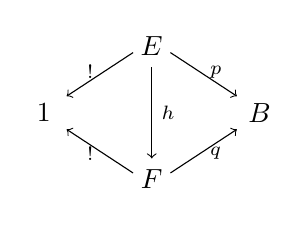
\begin{tikzpicture}[x=1.5em,y=1.5em]
  \node (E) at (2.6,1.6) {$E$};
  \node (o) at (0,0) {$1$};
  \node (B) at (5.2,0) {$B$};
  \node (F) at (2.6,-1.6) {$F$};
  \draw[->] (2.15,1.45) -- node[above,left,pos=0.45]{$\scriptstyle !$} (0.55,0.4);
  \draw[->] (3.05,1.45) -- node[above,right,pos=0.45]{$\scriptstyle p$} (4.65,0.4);
  \draw[->] (2.6,1.1) -- node[right,pos=0.5]{$\scriptstyle h$} (2.6,-1.1);
  \draw[->] (2.15,-1.45) -- node[below,left,pos=0.45]{$\scriptstyle !$} (0.55,-0.4);
  \draw[->] (3.05,-1.45) -- node[below,right,pos=0.45]{$\scriptstyle q$} (4.65,-0.4);
\end{tikzpicture}
\end{center}
\end{exercise}

\begin{exercise}\label{ex:mate-fibered-iso}
设 $A\xleftarrow{q}E\xrightarrow{p}B$ 与 $A\xleftarrow{s}F\xrightarrow{r}B$
是双侧纤维化，且 $\alpha\colon h\cong h'$ 是一个纤维化自然同构
\begin{center}
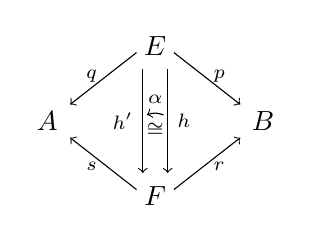
\begin{tikzpicture}[x=1.5em,y=1.5em]
  \node (E) at (2.6,1.8) {$E$};
  \node (A) at (0,0) {$A$};
  \node (B) at (5.2,0) {$B$};
  \node (F) at (2.6,-1.8) {$F$};
  \draw[->] (2.15,1.65) -- node[above,left,pos=0.45]{$\scriptstyle q$} (0.55,0.4);
  \draw[->] (3.05,1.65) -- node[above,right,pos=0.45]{$\scriptstyle p$} (4.65,0.4);
  \draw[->] (2.9,1.25) -- node[right,pos=0.5]{$\scriptstyle h$} (2.9,-1.25);
  \draw[->] (2.3,1.25) -- node[left,pos=0.5]{$\scriptstyle h'$} (2.3,-1.25);
  \draw[->] (2.8,0.15) to[bend right=20] node[above,pos=0.5]{$\scriptstyle\alpha$} node[below,pos=0.5]{$\scriptstyle\cong$} (2.4,0.15);
  \draw[->] (2.15,-1.65) -- node[below,left,pos=0.45]{$\scriptstyle s$} (0.55,-0.4);
  \draw[->] (3.05,-1.65) -- node[below,right,pos=0.45]{$\scriptstyle r$} (4.65,-0.4);
\end{tikzpicture}
\end{center}
使得 $r\alpha=\mathrm{id}_{p}$ 且 $s\alpha=\mathrm{id}_{q}$；特别地，$h$ 与
$h'$ 各自定义了一个跨度映射。证明：$h$ 是一个\trCartesianFunctor{}，当且仅当 $h'$ 是一个%
\trCartesianFunctor{}。
\end{exercise}
   %
\providecommand{\Cart}{\mathcal{C}art}
\providecommand{\coCart}{\mathrm{co}\mathcal{C}\mathit{art}}   %
\providecommand{\Fib}{\mathcal{F}ib}
\providecommand{\Fun}{\operatorname{Fun}}
\providecommand{\dashdownarrow}{\rotatebox[origin=c]{270}{$\dashrightarrow$}}   %

\section{双侧纤维化的∞-宇宙}\label{sec:two-sided-fibration-cosmos}

定理 7.1.4 与命题 7.1.7 的第一对等价条件，借助命题 6.3.14 的诸\trInfinityCosmos{}，%
为定义\trTwoSidedFibration{}的\trInfinityCosmos{}提供了两种等价的途径。

\begin{definition}[双侧纤维化的∞-宇宙]\label{def:two-sided-fibration-cosmos}
由定理 7.1.4 与命题 7.1.7，对\trInfinityCosmos{} $\mathcal{K}$ 中的任何一对%
\trInfinityCategory{} $A$ 与 $B$，$\mathcal{K}_{/A\times B}$ 的如下这对以%
\trQuasiCategory{}富集的子范畴
\begin{equation*}
\Cart(\coCart(\mathcal{K})_{/A})_{/\pi\colon A\times B\to A}
\qquad\text{与}\qquad
\coCart(\Cart(\mathcal{K})_{/B})_{/\pi\colon A\times B\to B}
\end{equation*}
相重合。我们记
\begin{equation*}
{}_{A\backslash}\Fib(\mathcal{K})_{/B}\subset\mathcal{K}_{/A\times B}
\end{equation*}
表示这一公共子范畴，并称之为从 $A$ 到 $B$ 的\textbf{\trTwoSidedFibration{}的%
\trInfinityCosmos}，如此称谓的理由稍后即明。

根据定义，从 $A\xleftarrow{q}E\xrightarrow{p}B$ 到
$A\xleftarrow{s}F\xrightarrow{r}B$ 的\trFunctorSpace
\begin{equation*}
\Fun_{{}_{A\backslash}\Fib(\mathcal{K})_{/B}}(E,F)
:=\Fun^{\mathrm{cart}}_{A\times B}(E,F)\subset\Fun_{A\times B}(E,F)
\end{equation*}
是由那些定义从 $E$ 到 $F$ 的\trCartesianFunctor{}的\trSpan{}映射构成的\trQuasiCategory%
（见命题 7.1.7）。

由于从 $A$ 到 $B$ 的\trTwoSidedIsofibration{}不过是 $A\times B$ 上的一个\trIsofibration{}，%
我们可以把 $\mathcal{K}_{/A\times B}$ 称作从 $A$ 到 $B$ 的\textbf{\trTwoSidedIsofibration{}的%
\trInfinityCosmos}。
\end{definition}

\begin{proposition}\label{prop:two-sided-fibration-cosmos-embedded}
对\trInfinityCosmos{} $\mathcal{K}$ 中的任何\trInfinityCategory{} $A$ 与
$B$，双侧\trFibration{}的\trInfinityCosmos{}
\[
{}_{A\backslash}\Fib(\mathcal{K})_{/B}\hookrightarrow\mathcal{K}_{/A\times B}
\]
在\trIsofibration{}的\trInfinityCosmos{}中是\trCosmologicallyEmbedded{}，
并由包含创生一个∞-宇宙结构。
\end{proposition}

\begin{proof}
该包含分解为
\begin{equation*}
\begin{array}{ccccc}
{}_{A\backslash}\Fib(\mathcal{K})_{/B} & & & & \mathcal{K}_{/A\times B}\\[0.4em]
\substack{\parallel\\ \wr} & & & & \substack{\parallel\\ \wr}\\[0.4em]
\coCart(\Cart(\mathcal{K})_{/B})_{/A\times B\to B}
& \hookrightarrow &
(\Cart(\mathcal{K})_{/B})_{/A\times B\to B}
& \hookrightarrow &
(\mathcal{K}_{/B})_{/A\times B\to B}
\end{array}
\end{equation*}
而由命题 6.3.14，两个包含都是\trCosmologicalEmbedding{}。
\end{proof}

\begin{observation}[双侧纤维化推广余/笛卡尔纤维化]\label{obs:two-sided-generalizes-cocartesian}
由练习 7.1.ii，从 $B$ 到 $1$ 的\trTwoSidedFibration{}是 $B$ 上的一个%
\trCocartesianFibration{}，而从 $1$ 到 $B$ 的\trTwoSidedFibration{}是 $B$ 上的一个%
\trCartesianFibration{}。实际上，作为\trInfinityCosmos{}，
\begin{equation*}
\coCart(\mathcal{K})_{/B}\cong{}_{B\backslash}\Fib(\mathcal{K})_{/1}
\qquad\text{与}\qquad
\Cart(\mathcal{K})_{/B}\cong{}_{1\backslash}\Fib(\mathcal{K})_{/B}.
\end{equation*}
在这个意义上，关于\trTwoSidedFibration{}的陈述同时推广了关于%
\trCartesianFibration{}与\trCocartesianFibration{}的陈述。
\end{observation}

现在我们转向先前许诺过的那些封闭性质：

\begin{proposition}\label{prop:pullback-restricts-two-sided}
对任何一对\trFunctor{} $a\colon A'\to A$ 与 $b\colon B'\to B$，\trCosmological{}%
拉回函子经限制而定义一个\trCosmologicalFunctor
\begin{center}
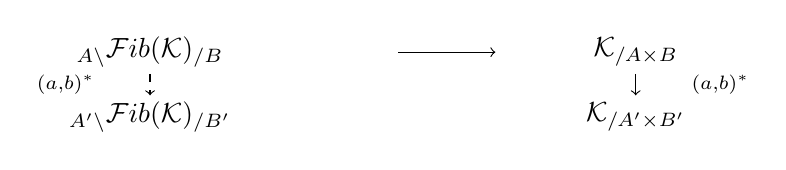
\begin{tikzpicture}[x=1.3em,y=1.3em]
  \node (TL) at (0,1.8) {${}_{A\backslash}\Fib(\mathcal{K})_{/B}$};
  \node (TR) at (13.5,1.8) {$\mathcal{K}_{/A\times B}$};
  \node (BL) at (0,0) {${}_{A'\backslash}\Fib(\mathcal{K})_{/B'}$};
  \node (BR) at (13.5,0) {$\mathcal{K}_{/A'\times B'}$};
  \draw[->] (6.9,1.8) -- (9.6,1.8);
  \draw[->,dashed] (0,1.2) -- (0,0.6);
  \node at (-2.35,0.9) {$\scriptstyle(a,b)^{*}$};
  \draw[->] (13.5,1.2) -- (13.5,0.6);
  \node at (15.85,0.9) {$\scriptstyle(a,b)^{*}$};
\end{tikzpicture}
\end{center}
特别地，一个\trTwoSidedFibration{}的拉回仍是一个\trTwoSidedFibration{}。
\end{proposition}

\begin{proof}
把函子 $(a,b)$ 分解为
$A'\times B'\xrightarrow{\mathrm{id}\times b}A'\times B\xrightarrow{a\times\mathrm{id}}A\times B$，%
可见每次考虑沿一侧作拉回就够了。命题 5.2.4 与练习 5.3.i 证明：沿
$b\colon B'\to B$ 的拉回保持\trCartesianFibration{}与\trCartesianFunctor{}，从而定义出一个%
限制后的函子
\begin{center}
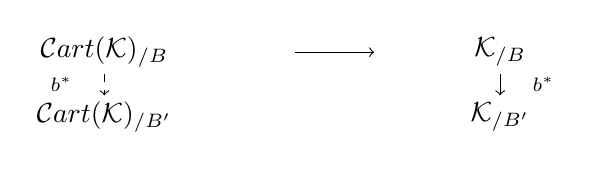
\begin{tikzpicture}[x=1.3em,y=1.3em]
  \node (TL) at (0,1.8) {$\Cart(\mathcal{K})_{/B}$};
  \node (TR) at (11,1.8) {$\mathcal{K}_{/B}$};
  \node (BL) at (0,0) {$\Cart(\mathcal{K})_{/B'}$};
  \node (BR) at (11,0) {$\mathcal{K}_{/B'}$};
  \draw[->] (5.3,1.8) -- (7.5,1.8);
  \draw[->,dashed] (0,1.2) -- (0,0.6);
  \node at (-1.2,0.9) {$\scriptstyle b^{*}$};
  \draw[->] (11,1.2) -- (11,0.6);
  \node at (12.2,0.9) {$\scriptstyle b^{*}$};
\end{tikzpicture}
\end{center}
由于 $\Cart(\mathcal{K})_{/B}$ 中的\trLimit{}与\trIsofibration{}是在
$\mathcal{K}_{/B}$ 中创生的，这一限制后的函子是\trCosmological{}（见引理 10.1.1）。
把这一结果应用于\trInfinityCosmos{} $\coCart(\mathcal{K})_{/A}$ 中的映射
\begin{center}
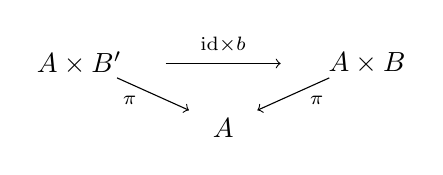
\begin{tikzpicture}[x=1.3em,y=1.3em]
  \node (L) at (0,1.8) {$A\times B'$};
  \node (R) at (8,1.8) {$A\times B$};
  \node (B) at (4,0) {$A$};
  \draw[->] (2.4,1.8) -- (5.6,1.8);
  \node at (4,2.32) {$\scriptstyle\mathrm{id}\times b$};
  \draw[->] (1.05,1.4) -- (3.05,0.5);
  \node at (1.4,0.78) {$\scriptstyle\pi$};
  \draw[->] (6.95,1.4) -- (4.95,0.5);
  \node at (6.6,0.78) {$\scriptstyle\pi$};
\end{tikzpicture}
\end{center}
我们得出：拉回经限制而定义一个\trCosmologicalFunctor
\begin{equation*}
\begin{array}{ccccc}
\Cart(\coCart(\mathcal{K})_{/A})_{/\pi\colon A\times B\to A}
& \hookrightarrow &
(\coCart(\mathcal{K})_{/A})_{/\pi\colon A\times B\to A}
& \hookrightarrow &
\mathcal{K}_{/A\times B}\\[0.5em]
{}_{(\mathrm{id}\times b)^{*}}\dashdownarrow & &
\dashdownarrow_{(\mathrm{id}\times b)^{*}} & &
\downarrow_{(\mathrm{id}\times b)^{*}}\\[0.5em]
\Cart(\coCart(\mathcal{K})_{/A})_{/\pi\colon A\times B'\to A}
& \hookrightarrow &
(\coCart(\mathcal{K})_{/A})_{/\pi\colon A\times B'\to A}
& \hookrightarrow &
\mathcal{K}_{/A\times B'}
\end{array}
\end{equation*}
\end{proof}

\begin{lemma}\label{lem:whiskering-two-sided-fibrations}
若 $A\xleftarrow{q}E\xrightarrow{p}B$ 是从 $A$ 到 $B$ 的一个\trTwoSidedFibration{}，%
$v\colon A\twoheadrightarrow C$ 是一个\trCocartesianFibration{}而
$u\colon B\twoheadrightarrow D$ 是一个\trCartesianFibration{}，那么复合\trSpan
\begin{equation*}
C\xleftarrow{v}A\xleftarrow{q}E\xrightarrow{p}B\xrightarrow{u}D
\end{equation*}
定义一个从 $C$ 到 $D$ 的\trTwoSidedFibration{}。此外，从 $A$ 到 $B$ 的%
\trTwoSidedFibration{}之间的一个\trCartesianFunctor $h$ 诱导出从 $C$ 到 $D$ 的%
\trTwoSidedFibration{}之间的一个\trCartesianFunctor{}：
\begin{center}
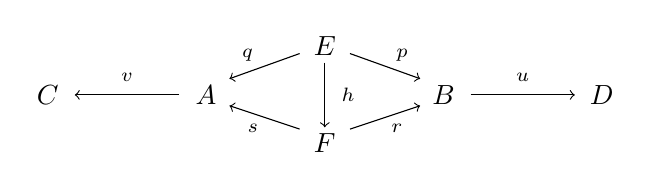
\begin{tikzpicture}[x=1.3em,y=1.3em]
  \node (E) at (3.3,2.7) {$E$};
  \node (A) at (0,1.35) {$A$};
  \node (B) at (6.6,1.35) {$B$};
  \node (C) at (-4.4,1.35) {$C$};
  \node (D) at (11,1.35) {$D$};
  \node (F) at (3.3,0) {$F$};
  \draw[->] (2.6,2.5) -- (0.65,1.8);
  \node at (1.15,2.45) {$\scriptstyle q$};
  \draw[->] (4.0,2.5) -- (5.95,1.8);
  \node at (5.45,2.45) {$\scriptstyle p$};
  \draw[->] (3.3,2.25) -- (3.3,0.45);
  \node at (3.95,1.35) {$\scriptstyle h$};
  \draw[->] (-0.75,1.35) -- (-3.65,1.35);
  \node at (-2.2,1.85) {$\scriptstyle v$};
  \draw[->] (7.35,1.35) -- (10.25,1.35);
  \node at (8.8,1.85) {$\scriptstyle u$};
  \draw[->] (2.6,0.4) -- (0.65,1.05);
  \node at (1.3,0.42) {$\scriptstyle s$};
  \draw[->] (4.0,0.4) -- (5.95,1.05);
  \node at (5.3,0.42) {$\scriptstyle r$};
\end{tikzpicture}
\end{center}
这一\trWhiskering{}复合并不定义一个从 ${}_{A\backslash}\Fib(\mathcal{K})_{/B}$ 到
${}_{C\backslash}\Fib(\mathcal{K})_{/D}$ 的\trCosmologicalFunctor{}，因为由与等价%
纤维化 $v\times u$ 作复合所定义的函子
$(v\times u)_{*}\colon\mathcal{K}_{/A\times B}\to\mathcal{K}_{/C\times D}$
并不保持\trFlexibleWeightedLimit{}（见非例 1.3.6）。
\end{lemma}

\begin{proof}
由定理 7.1.4，逐侧分别考虑复合即可，比如说与一个\trCocartesianFibration{}
$v\colon A\twoheadrightarrow C$ 复合。在\trInfinityCosmos{} $\Cart(\mathcal{K})_{/B}$
中工作，我们手头有\trCocartesianFibration
\begin{center}
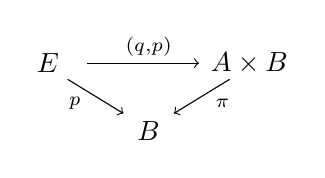
\begin{tikzpicture}[x=1.3em,y=1.3em]
  \node (E) at (0,1.9) {$E$};
  \node (AB) at (5.6,1.9) {$A\times B$};
  \node (B) at (2.8,0) {$B$};
  \draw[->] (1.1,1.9) -- (4.2,1.9);
  \node at (2.8,2.36) {$\scriptstyle(q,p)$};
  \draw[->] (0.55,1.45) -- (2.1,0.5);
  \node at (0.75,0.78) {$\scriptstyle p$};
  \draw[->] (5.05,1.45) -- (3.5,0.5);
  \node at (4.85,0.78) {$\scriptstyle\pi$};
\end{tikzpicture}
\qquad
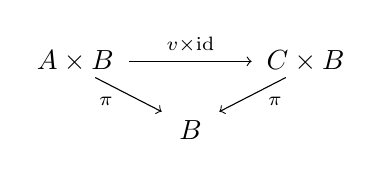
\begin{tikzpicture}[x=1.3em,y=1.3em]
  \node (AB) at (0,1.9) {$A\times B$};
  \node (CB) at (6.4,1.9) {$C\times B$};
  \node (B) at (3.2,0) {$B$};
  \draw[->] (1.5,1.9) -- (4.9,1.9);
  \node at (3.2,2.36) {$\scriptstyle v\times\mathrm{id}$};
  \draw[->] (0.55,1.45) -- (2.4,0.5);
  \node at (0.85,0.78) {$\scriptstyle\pi$};
  \draw[->] (5.85,1.45) -- (4.0,0.5);
  \node at (5.55,0.78) {$\scriptstyle\pi$};
\end{tikzpicture}
\end{center}
它们复合起来定义一个\trCocartesianFibration
\begin{center}
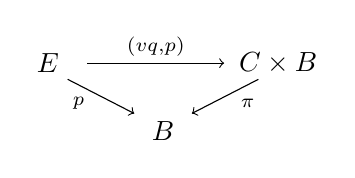
\begin{tikzpicture}[x=1.3em,y=1.3em]
  \node (E) at (0,1.9) {$E$};
  \node (CB) at (6.4,1.9) {$C\times B$};
  \node (B) at (3.2,0) {$B$};
  \draw[->] (1.1,1.9) -- (4.9,1.9);
  \node at (3.0,2.36) {$\scriptstyle(vq,p)$};
  \draw[->] (0.55,1.45) -- (2.4,0.5);
  \node at (0.85,0.78) {$\scriptstyle p$};
  \draw[->] (5.85,1.45) -- (4.0,0.5);
  \node at (5.55,0.78) {$\scriptstyle\pi$};
\end{tikzpicture}
\end{center}
从而如所愿地定义一个从 $C$ 到 $B$ 的\trTwoSidedFibration{}。

由引理 5.2.3，诸 $vq$-\trCocartesian\trCell{}恰是诸 $v$-\trCocartesian\trCell{}的%
$q$-\trCocartesian{}提升。若 $h$ 是从 $q$ 到 $s$ 的一个\trCartesianFunctor{}，那么这些%
\trCell{}显然被保持，这就证明了 $h$ 也定义一个从 $vq$ 到 $vs$ 的\trCartesianFunctor{}。由%
命题 7.1.7(iv)，这就证明了 $h$ 在须化后的\trTwoSidedFibration{}之间定义一个%
\trCartesianFunctor{}。
\end{proof}

\cref{prop:pullback-restricts-two-sided}与\cref{lem:whiskering-two-sided-fibrations}%
结合起来证明：\trTwoSidedFibration{}可以「水平地」复合。

\begin{proposition}\label{prop:horizontal-composite-two-sided}
从 $A$ 到 $B$ 的一个\trTwoSidedFibration{}沿一个从 $B$ 到 $C$ 的%
\trTwoSidedFibration{}的拉回，定义一个从 $A$ 到 $C$ 的\trTwoSidedFibration{}，%
如下列所示：
\begin{center}
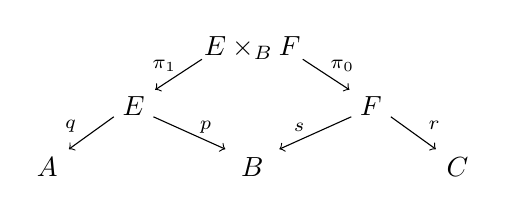
\begin{tikzpicture}[x=1.3em,y=1.3em]
  \node (P) at (3.3,3.3) {$E\times_{B}F$};
  \node (E) at (0,1.7) {$E$};
  \node (F) at (6.6,1.7) {$F$};
  \node (A) at (-2.4,0) {$A$};
  \node (B) at (3.3,0) {$B$};
  \node (C) at (9.0,0) {$C$};
  \draw[->] (1.9,3.0) -- (0.6,2.15);
  \node at (0.85,2.82) {$\scriptstyle\pi_{1}$};
  \draw[->] (4.7,3.0) -- (6.0,2.15);
  \node at (5.8,2.82) {$\scriptstyle\pi_{0}$};
  \draw[->] (-0.55,1.4) -- (-1.8,0.5);
  \node at (-1.75,1.15) {$\scriptstyle q$};
  \draw[->] (0.55,1.4) -- (2.55,0.5);
  \node at (2.0,1.12) {$\scriptstyle p$};
  \draw[->] (6.05,1.4) -- (4.05,0.5);
  \node at (4.6,1.12) {$\scriptstyle s$};
  \draw[->] (7.15,1.4) -- (8.4,0.5);
  \node at (8.35,1.15) {$\scriptstyle r$};
\end{tikzpicture}
\end{center}
\end{proposition}

\begin{proof}
该复合\trTwoSidedFibration{}分两个阶段构造：首先作拉回
\begin{center}
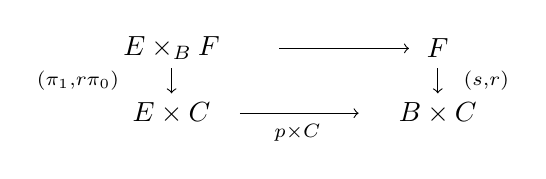
\begin{tikzpicture}[x=1.3em,y=1.3em]
  \node (TL) at (0,1.8) {$E\times_{B}F$};
  \node (TR) at (7.4,1.8) {$F$};
  \node (BL) at (0,0) {$E\times C$};
  \node (BR) at (7.4,0) {$B\times C$};
  \draw[->] (3.0,1.8) -- (6.6,1.8);
  \draw[->] (0,1.25) -- (0,0.55);
  \node at (-2.6,0.9) {$\scriptstyle(\pi_{1},r\pi_{0})$};
  \draw[->] (7.4,1.25) -- (7.4,0.55);
  \node at (8.75,0.9) {$\scriptstyle(s,r)$};
  \draw[->] (1.9,0) -- (5.2,0);
  \node at (3.5,-0.55) {$\scriptstyle p\times C$};
  \node at (1.1,1.1) {$\scriptstyle\lrcorner$};
\end{tikzpicture}
\end{center}
然后将左腿与\trCocartesianFibration{} $q\colon E\twoheadrightarrow A$ 复合。由%
\cref{prop:pullback-restricts-two-sided}与\cref{lem:whiskering-two-sided-fibrations}，%
其结果是一个从 $A$ 到 $C$ 的\trTwoSidedFibration{}。或者，该复合也可以这样构造：%
沿 $A\times s$ 作拉回并与\trCartesianFibration{} $r\colon F\twoheadrightarrow C$
复合，得到另一个从 $A$ 到 $C$ 的\trTwoSidedFibration{}，它与第一个典范同构。
\end{proof}

有了这些结果，我们便可以为我们的例子库增添几个新成员了：

\begin{example}\label{exa:two-sided-fibration-from-cart-cocart}
若 $p\colon E\twoheadrightarrow B$ 是一个\trCartesianFibration{}而
$q\colon F\twoheadrightarrow A$ 是一个\trCocartesianFibration{}，那么由与积投影%
复合而成的\trSpan
\begin{equation*}
A\overset{q}{\twoheadleftarrow}F\overset{\pi}{\twoheadleftarrow}F\times E\overset{\pi}{\twoheadrightarrow}E\overset{p}{\twoheadrightarrow}B
\end{equation*}
依练习 7.1.i 定义一个从 $A$ 到 $B$ 的\trTwoSidedFibration{}。
\end{example}

\begin{example}\label{exa:comma-span-two-sided}
由命题 7.1.6 与\cref{prop:pullback-restricts-two-sided}，一般的逗号\trSpan
\begin{equation*}
C\xleftarrow{p_{1}}\mathrm{Hom}_{A}(f,g)\xrightarrow{p_{0}}B
\end{equation*}
是一个\trTwoSidedFibration{}，因为它是
$A\overset{p_{1}}{\twoheadleftarrow}A^{2}\overset{p_{0}}{\twoheadrightarrow}A$
的一个\trPullback{}。
\end{example}

\begin{example}\label{exa:horizontal-composite-comma-spans}
由\cref{prop:horizontal-composite-two-sided}与\cref{exa:comma-span-two-sided}，%
逗号\trSpan{}的水平复合也是\trTwoSidedFibration{}。例如，\trTwoSidedFibration
\begin{equation*}
A\overset{p_{1}}{\twoheadleftarrow}A^{2}
\overset{p_{n+1}}{\twoheadleftarrow}A^{n+1}
\overset{p_{0}}{\twoheadrightarrow}A
\end{equation*}
是箭头\trSpan{}
$A\overset{p_{1}}{\twoheadleftarrow}A^{2}\overset{p_{0}}{\twoheadrightarrow}A$
的 $n$ 元水平复合。
\end{example}

其他值得注意的\trTwoSidedFibration{}还包括逗号\trSpan{}的水平复合，其特例之一%
将在下一节中占据显要地位。
   %
\providecommand{\qcor}[1]{\ulcorner#1\urcorner}   %
\providecommand{\qcOne}{\mathbf{1}}   %
\providecommand{\evid}[1]{\mathrm{ev}_{\qcor{\mathrm{id}_{#1}}}}   %

\subsection*{练习}

\begin{exercise}\label{ex:pullback-cartesian-functors}
考虑一张图表，其中 $h$ 与 $k$ 分别在从 $A$ 到 $B$ 的诸\trTwoSidedFibration{}%
之间、以及从 $B$ 到 $C$ 的诸\trTwoSidedFibration{}之间定义\trCartesianFunctor{}：
\begin{center}
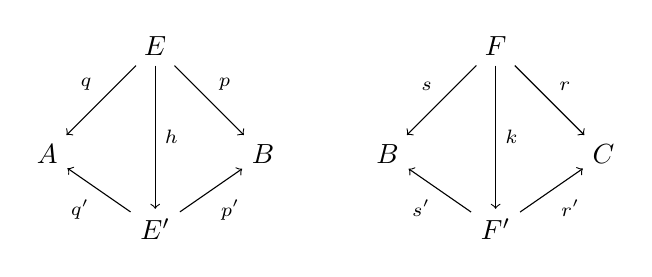
\begin{tikzpicture}[x=1.5em,y=1.5em]
  \begin{scope}[shift={(0,0)}]
    \node (E)  at (0,1.6) {$E$};
    \node (A)  at (-2.6,-1.0) {$A$};
    \node (B)  at (2.6,-1.0) {$B$};
    \node (Ep) at (0,-2.8) {$E'$};
    \draw[->] (E) -- node[above left]{$\scriptstyle q$} (A);
    \draw[->] (E) -- node[above right]{$\scriptstyle p$} (B);
    \draw[->] (E) -- node[right]{$\scriptstyle h$} (Ep);
    \draw[->] (Ep) -- node[below left]{$\scriptstyle q'$} (A);
    \draw[->] (Ep) -- node[below right]{$\scriptstyle p'$} (B);
  \end{scope}
  \begin{scope}[shift={(8.2,0)}]
    \node (F)  at (0,1.6) {$F$};
    \node (B2) at (-2.6,-1.0) {$B$};
    \node (C)  at (2.6,-1.0) {$C$};
    \node (Fp) at (0,-2.8) {$F'$};
    \draw[->] (F) -- node[above left]{$\scriptstyle s$} (B2);
    \draw[->] (F) -- node[above right]{$\scriptstyle r$} (C);
    \draw[->] (F) -- node[right]{$\scriptstyle k$} (Fp);
    \draw[->] (Fp) -- node[below left]{$\scriptstyle s'$} (B2);
    \draw[->] (Fp) -- node[below right]{$\scriptstyle r'$} (C);
  \end{scope}
\end{tikzpicture}
\end{center}
证明：$h$ 与 $k$ 经\trPullback{}可定义出一个介于从 $A$ 到 $C$ 的%
\trTwoSidedFibration{}之间的\trCartesianFunctor
$(h,k)\colon E\times_{B}F\to E'\times_{B}F'$。
\end{exercise}

\section{双侧 Yoneda 引理}\label{sec:two-sided-yoneda-lemma}

在本节中，我们将证明\trYonedaLemma{}的一个双侧版本，所借助的是可表示双侧纤维化%
的如下概念：

\begin{definition}\label{def:represented-two-sided-fibration}
对\trGeneralizedElement{}的任意一个跨度
$A\overset{a}{\leftarrow}X\overset{b}{\rightarrow}B$，如下跨度
\begin{center}
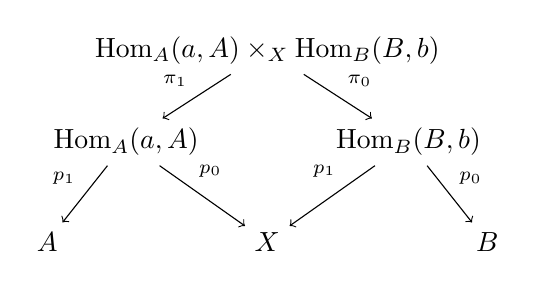
\begin{tikzpicture}[x=1.5em,y=1.5em]
  \node (P)  at (3.4,2.6) {$\mathrm{Hom}_{A}(a,A)\times_{X}\mathrm{Hom}_{B}(B,b)$};
  \node (HA) at (0,0.4) {$\mathrm{Hom}_{A}(a,A)$};
  \node (HB) at (6.8,0.4) {$\mathrm{Hom}_{B}(B,b)$};
  \node (A)  at (-1.9,-2.0) {$A$};
  \node (X)  at (3.4,-2.0) {$X$};
  \node (B)  at (8.7,-2.0) {$B$};
  \draw[->] (P) -- node[above left]{$\scriptstyle\pi_{1}$} (HA);
  \draw[->] (P) -- node[above right]{$\scriptstyle\pi_{0}$} (HB);
  \node at (3.4,1.5) {$\scriptstyle\llcorner$};
  \draw[->] (HA) -- node[above left]{$\scriptstyle p_{1}$} (A);
  \draw[->] (HA) -- node[above right,pos=0.35]{$\scriptstyle p_{0}$} (X);
  \draw[->] (HB) -- node[above left,pos=0.35]{$\scriptstyle p_{1}$} (X);
  \draw[->] (HB) -- node[above right]{$\scriptstyle p_{0}$} (B);
\end{tikzpicture}
\end{center}
定义了从 $A$ 到 $B$ 的一条\trTwoSidedFibration{}，我们称之为\textbf{由 $a$ 与 $b$
表示的双侧纤维化}（two-sided fibration represented by $a$ and $b$）。与单侧可%
表示物的情形一样，在 $(a,b)\colon X\to A\times B$ 之上的\trFiber{}中存在一个
典范的\trGeneralizedElement{}
$(\qcor{\mathrm{id}_{a}},\qcor{\mathrm{id}_{b}})\colon X\to\mathrm{Hom}_{A}(a,A)\times_{X}\mathrm{Hom}_{B}(B,b)$。
\end{definition}

\cref{def:represented-two-sided-fibration}的这一术语由双侧纤维化的那个%
\trYonedaLemma{}所证成，而后者我们将使用\cref{cor:generalized-yoneda-lemma}的
广义元素之\trYonedaLemma{}来证明。

\begin{theorem}[\trYonedaLemma]\label{thm:two-sided-yoneda-lemma}
对任意跨度 $A\overset{a}{\leftarrow}X\overset{b}{\rightarrow}B$ 与任意%
\trTwoSidedFibration{}
$A\overset{q}{\twoheadleftarrow}E\overset{p}{\twoheadrightarrow}B$，沿元素
$(\qcor{\mathrm{id}_{a}},\qcor{\mathrm{id}_{b}})\colon X\to\mathrm{Hom}_{A}(a,A)\times_{X}\mathrm{Hom}_{B}(B,b)$ 的限制定义了%
\trQuasiCategory{}之间的一个\trEquivalence
{\small\[
\mathrm{Fun}_{A\times B}^{\mathrm{cart}}\!\left(
\begin{gathered}
\mathrm{Hom}_{A}(a,A)\times_{X}\mathrm{Hom}_{B}(B,b)\\[-2pt]
\downarrow\scriptstyle (p_{1}\pi_{1},\,p_{0}\pi_{0})\\[-2pt]
A\times B
\end{gathered}
\;\right.,
\left.
\begin{gathered}
E\\[-2pt]
\downarrow\scriptstyle (q,\,p)\\[-2pt]
A\times B
\end{gathered}
\right)
\xrightarrow[\ \sim\ ]{\ \mathrm{ev}_{(\qcor{\mathrm{id}_{a}},\,\qcor{\mathrm{id}_{b}})}\ }
\mathrm{Fun}_{A\times B}\!\left(
\begin{gathered}
X\\[-2pt]
\downarrow\scriptstyle (a,\,b)\\[-2pt]
A\times B
\end{gathered}
\;\right.,
\left.
\begin{gathered}
E\\[-2pt]
\downarrow\scriptstyle (q,\,p)\\[-2pt]
A\times B
\end{gathered}
\right)
\]}
\end{theorem}

\begin{proof}
我们以定理 7.1.4(i) 的视角来证明这一结果：在∞-宇宙 $\mathcal{K}$ 中，把作为靶子
的\trTwoSidedFibration{}
$A\overset{q}{\twoheadleftarrow}E\overset{p}{\twoheadrightarrow}B$ 视为
∞-宇宙 $\mathrm{co}\mathcal{C}\mathit{art}(\mathcal{K})_{/A}$\footnote{原书印作 $\mathrm{co}\mathcal{C}\mathit{art}(\mathcal{K})_{/A\times B}$，按定理 7.1.4(i) 与下文自述应为 $\mathrm{co}\mathcal{C}\mathit{art}(\mathcal{K})_{/A}$，此处径改。——译者注}中
$\pi\colon A\times B\twoheadrightarrow A$ 之上的一条\trCartesianFibration{}。我们
通过两次施用\cref{cor:generalized-yoneda-lemma}来推导这一结果：先对
$\mathrm{co}\mathcal{C}\mathit{art}(\mathcal{K})_{/A}$ 中 $\pi\colon A\times B\twoheadrightarrow A$
之上的诸\trCartesianFibration{}施用，再对 $\mathcal{K}$ 中 $A$ 之上的诸%
\trCocartesianFibration{}施用。

为给 Yoneda 引理的第一次应用做准备，我们需要在 $\mathrm{co}\mathcal{C}\mathit{art}(\mathcal{K})_{/A}$
中，从 $A$ 之上的映射
\begin{rveq}\label{eq:span-over-a}
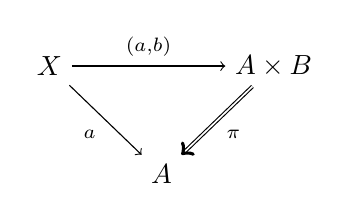
\begin{tikzpicture}[x=1.5em,y=1.5em]
  \node (X)  at (0,1.3) {$X$};
  \node (AB) at (5.4,1.3) {$A\times B$};
  \node (A)  at (2.7,-1.3) {$A$};
  \draw[->] (X) -- node[above]{$\scriptstyle(a,b)$} (AB);
  \draw[->] (X) -- node[below left]{$\scriptstyle a$} (A);
  \draw[double,->] (AB) -- node[below right]{$\scriptstyle\pi$} (A);
\end{tikzpicture}
\end{rveq}
出发，造出一个余定义域为 $\pi\colon A\times B\twoheadrightarrow A$ 的%
\trGeneralizedElement{}。\cref{cor:generalized-yoneda-lemma}给出一个\trEquivalence
\[
\mathrm{Fun}_{A}^{\mathrm{cart}}\bigl(
\mathrm{Hom}_{A}(a,A)\mathrel{\overset{p_{1}}{\twoheadrightarrow}}A,\,
A\times B\mathrel{\overset{\pi}{\twoheadrightarrow}}A
\bigr)
\xrightarrow[\ \sim\ ]{\ \mathrm{ev}_{\qcor{\mathrm{id}_{a}}}\ }
\mathrm{Fun}_{A}\bigl(
X\xrightarrow{\ a\ }A,\,
A\times B\mathrel{\overset{\pi}{\twoheadrightarrow}}A
\bigr)
\]
它告诉我们：$a\colon X\to A$ 在 $\mathrm{co}\mathcal{C}\mathit{art}(\mathcal{K})_{/A}$ 中的反射由
$p_{1}\colon\mathrm{Hom}_{A}(a,A)\twoheadrightarrow A$ 给出。于是我们取广义元素
为诸\trCocartesianFibration{}之间的如下\trCartesianFunctor
\begin{rveq}\label{eq:cartesian-functor-pair}
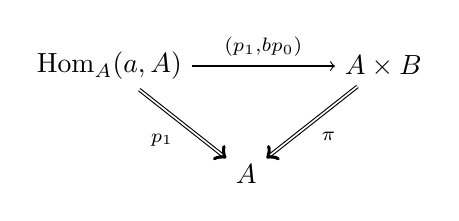
\begin{tikzpicture}[x=1.5em,y=1.5em]
  \node (H)  at (0,1.3) {$\mathrm{Hom}_{A}(a,A)$};
  \node (AB) at (6.6,1.3) {$A\times B$};
  \node (A)  at (3.3,-1.3) {$A$};
  \draw[->] (H) -- node[above]{$\scriptstyle(p_{1},bp_{0})$} (AB);
  \draw[double,->] (H) -- node[below left]{$\scriptstyle p_{1}$} (A);
  \draw[double,->] (AB) -- node[below right]{$\scriptstyle\pi$} (A);
\end{tikzpicture}
\end{rveq}
它沿 $\qcor{\mathrm{id}_{a}}\colon X\to\mathrm{Hom}_{A}(a,A)$ 的限制即
\eqref{eq:span-over-a}。

由\cref{cor:generalized-yoneda-lemma}再一次，对象 \eqref{eq:cartesian-functor-pair}
从 $(\mathrm{co}\mathcal{C}\mathit{art}(\mathcal{K})_{/A})_{/\pi\colon A\times B\twoheadrightarrow A}$
到 ${}_{A\backslash}\mathcal{F}\mathit{ib}(\mathcal{K})_{/B}$ 的反射，由其右逗号表示%
（该表示形成于 $\mathrm{co}\mathcal{C}\mathit{art}(\mathcal{K})_{/A}$ 中）的余定义域投影给出。这
复原出\trTwoSidedFibration
\begin{center}
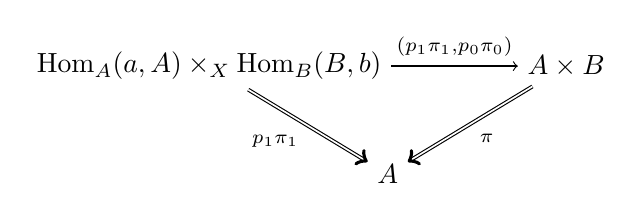
\begin{tikzpicture}[x=1.5em,y=1.5em]
  \node (P)  at (0,1.3) {$\mathrm{Hom}_{A}(a,A)\times_{X}\mathrm{Hom}_{B}(B,b)$};
  \node (AB) at (8.6,1.3) {$A\times B$};
  \node (A)  at (4.3,-1.3) {$A$};
  \draw[->] (P) -- node[above]{$\scriptstyle(p_{1}\pi_{1},p_{0}\pi_{0})$} (AB);
  \draw[double,->] (P) -- node[below left]{$\scriptstyle p_{1}\pi_{1}$} (A);
  \draw[double,->] (AB) -- node[below right]{$\scriptstyle\pi$} (A);
\end{tikzpicture}
\end{center}
于是，该结果给出一个\trEquivalence
{\small\[
\mathrm{Fun}_{A\times B}^{\mathrm{cart}}\!\left(
\begin{gathered}
\mathrm{Hom}_{A}(a,A)\times_{X}\\[-2pt]
\mathrm{Hom}_{B}(B,b)\\[-2pt]
\downarrow\scriptstyle (p_{1}\pi_{1},\,p_{0}\pi_{0})\\[-2pt]
A\times B
\end{gathered}
\;\right.,
\left.
\begin{gathered}
E\\[-2pt]
\downarrow\scriptstyle (q,\,p)\\[-2pt]
A\times B
\end{gathered}
\right)
\xrightarrow[\ \sim\ ]{\ \mathrm{ev}_{(\qcor{\mathrm{id}_{a}},\,\qcor{bp_{0}})}\ }
\mathrm{Fun}_{A\times B}^{\mathrm{cart}}\!\left(
\begin{gathered}
\mathrm{Hom}_{A}(a,A)\\[-2pt]
\downarrow\scriptstyle (p_{1},\,bp_{0})\\[-2pt]
A\times B
\end{gathered}
\;\right.,
\left.
\begin{gathered}
E\\[-2pt]
\downarrow\scriptstyle (q,\,p)\\[-2pt]
A\times B
\end{gathered}
\;\right)
\]}
其中右边的\trFunctorSpace{}由 $\mathrm{co}\mathcal{C}\mathit{art}(\mathcal{K})_{/A}$ 中%
\trFunctorSpace{}的如下\trPullback{}定义
\begin{center}
\begin{tikzpicture}[x=1.3em,y=1.3em,every node/.style={font=\small}]
  \node (NW) at (0,1.7) {$\mathrm{Fun}_{A\times B}^{\mathrm{cart}}\bigl(\mathrm{Hom}_{A}(a,A),\,E\bigr)$};
  \node (NE) at (10.4,1.7) {$\mathrm{Fun}_{A}^{\mathrm{cart}}\bigl(\mathrm{Hom}_{A}(a,A)\mathrel{\overset{p_{1}}{\twoheadrightarrow}}A,\,E\mathrel{\overset{q}{\twoheadrightarrow}}A\bigr)$};
  \node (SW) at (0,-1.7) {$\qcOne$};
  \node (SE) at (10.4,-1.7) {$\mathrm{Fun}_{A}^{\mathrm{cart}}\bigl(\mathrm{Hom}_{A}(a,A)\mathrel{\overset{p_{1}}{\twoheadrightarrow}}A,\,A\times B\mathrel{\overset{\pi}{\twoheadrightarrow}}A\bigr)$};
  \draw[->] (NW) -- (NE);
  \draw[->] (NW) -- (SW);
  \draw[->] (SW) -- node[above,pos=0.28]{$\scriptstyle(p_{1},bp_{0})$} (SE);
  \draw[->] (NE) -- node[right]{$\scriptstyle(q,p)_{*}$} (SE);
  \node at (0.5,0.9) {$\scriptstyle\llcorner$};
\end{tikzpicture}
\end{center}
\cref{cor:generalized-yoneda-lemma}又一次给出自然等价
\begin{center}
\begin{tikzpicture}[x=1.2em,y=1.3em,every node/.style={font=\small}]
  \node (TL) at (0,1.7) {$\mathrm{Fun}_{A}^{\mathrm{cart}}\bigl(\mathrm{Hom}_{A}(a,A)\mathrel{\overset{p_{1}}{\twoheadrightarrow}}A,\,E\mathrel{\overset{q}{\twoheadrightarrow}}A\bigr)$};
  \node (TR) at (10.6,1.7) {$\mathrm{Fun}_{A}\bigl(X\xrightarrow{\ a\ }A,\,E\mathrel{\overset{q}{\twoheadrightarrow}}A\bigr)$};
  \node (BL) at (0,-1.7) {$\mathrm{Fun}_{A}^{\mathrm{cart}}\bigl(\mathrm{Hom}_{A}(a,A)\mathrel{\overset{p_{1}}{\twoheadrightarrow}}A,\,A\times B\mathrel{\overset{\pi}{\twoheadrightarrow}}A\bigr)$};
  \node (BR) at (10.6,-1.7) {$\mathrm{Fun}_{A}\bigl(X\xrightarrow{\ a\ }A,\,A\times B\mathrel{\overset{\pi}{\twoheadrightarrow}}A\bigr)$};
  \draw[->] (TL) -- node[above]{$\scriptstyle\mathrm{ev}_{\qcor{\mathrm{id}_{a}}}$} node[below]{$\scriptstyle\sim$} (TR);
  \draw[->] (BL) -- node[above]{$\scriptstyle\mathrm{ev}_{\qcor{\mathrm{id}_{a}}}$} node[below]{$\scriptstyle\sim$} (BR);
  \draw[->] (TL) -- node[left]{$\scriptstyle(q,p)_{*}$} (BL);
  \draw[->] (TR) -- node[right]{$\scriptstyle(q,p)_{*}$} (BR);
\end{tikzpicture}
\end{center}
它们诱导出：左手边的\trIsofibration{}在 $(p_{1},bp_{0})$ 之上的\trFiber{}与
右手边的\trIsofibration{}在
$(p_{1},bp_{0})\cdot\qcor{\mathrm{id}_{a}}=(a,b)$ 之上的\trFiber{}之间的一个%
\trEquivalence{}。为计算这一\trFiber{}，请注意右手边的\trIsofibration{}本身就是
如下\trPullback
\begin{center}
\begin{tikzpicture}[x=1.35em,y=1.35em,every node/.style={font=\small}]
  \node (F1) at (0,1.8)  {$\mathrm{Fun}_{A\times B}(X,E)$};
  \node (F2) at (5.2,1.8)  {$\mathrm{Fun}_{A}(X,E)$};
  \node (F3) at (10.6,1.8) {$\mathrm{Fun}(X,E)$};
  \node (u1) at (0,-0.2)  {$\qcOne$};
  \node (G2) at (5.2,-0.2)  {$\mathrm{Fun}_{A}(X,A\times B)$};
  \node (G3) at (10.6,-0.2) {$\mathrm{Fun}(X,A\times B)$};
  \node (u2) at (0,-2.6)  {$\qcOne$};
  \node (FA) at (7.6,-2.6) {$\mathrm{Fun}(X,A)$};
  \draw[->] (F1) -- (F2);
  \draw[->] (F2) -- (F3);
  \draw[->] (u1) -- node[above]{$\scriptstyle(a,b)$} (G2);
  \draw[->] (G2) -- (G3);
  \draw[->] (u2) -- node[below,pos=0.3]{$\scriptstyle a$} (FA);
  \draw[->] (F2) -- node[left]{$\scriptstyle(q,p)_{*}$} (G2);
  \draw[->] (F3) -- node[right]{$\scriptstyle(q,p)$} (G3);
  \draw[->] (G3) -- node[right]{$\scriptstyle\pi_{*}$} (FA);
  \draw[->] (F3.south west) -- node[left,pos=0.55]{$\scriptstyle q_{*}$} (FA.north east);
  \draw[->] (G2) -- (u2);
  \draw[->,dashed] (u1) to[out=38,in=-115] (F1);
  \node at (0.55,0.95) {$\scriptstyle\llcorner$};
  \node at (5.75,-1.15) {$\scriptstyle\llcorner$};
\end{tikzpicture}
\end{center}
复合得出的\trEquivalence{}即为与典范\trGeneralizedElement{}作\trPreComposition{}所定义的那个
映射，证明由此完成。
\begin{center}
\begin{tikzpicture}[x=1.3em,y=1.3em,every node/.style={font=\small}]
  \node (TL) at (0,1.7) {$\mathrm{Fun}_{A\times B}^{\mathrm{cart}}\bigl(\mathrm{Hom}_{A}(a,A)\times_{X}\mathrm{Hom}_{B}(B,b),\,E\bigr)$};
  \node (TR) at (11.0,1.7) {$\mathrm{Fun}_{A\times B}^{\mathrm{cart}}\bigl(\mathrm{Hom}_{A}(a,A),\,E\bigr)$};
  \node (BR) at (11.0,-1.7) {$\mathrm{Fun}_{A\times B}(X,\,E)$};
  \draw[->] (TL) -- node[above]{$\scriptstyle\mathrm{ev}_{(\qcor{\mathrm{id}_{a}},\,\qcor{bp_{0}})}$} node[below]{$\scriptstyle\sim$} (TR);
  \draw[->] (TL) -- node[below left,pos=0.55]{$\scriptstyle\mathrm{ev}_{(\qcor{\mathrm{id}_{a}},\,\qcor{\mathrm{id}_{b}})}$} node[above left,pos=0.45]{$\scriptstyle\sim$} (BR);
  \draw[->] (TR) -- node[right]{$\scriptstyle\mathrm{ev}_{\qcor{\mathrm{id}_{a}}}$} (BR);
\end{tikzpicture}
\end{center}
\end{proof}

与\cref{cor:generalized-yoneda-lemma}一样，我们把\cref{thm:two-sided-yoneda-lemma}
解读为：它为双侧纤维化这一子范畴的包含定义了一个左双伴随，把跨度
$A\overset{a}{\leftarrow}X\overset{b}{\rightarrow}B$ 送到%
\cref{def:represented-two-sided-fibration}中所构造的那条\trTwoSidedIsofibration{}。当跨度
由单个非恒同\trFunctor{}表示时，人们也许会更青睐\cref{thm:two-sided-yoneda-lemma}
的一个「单侧」版本——它的确立要简单得多：

   %
\providecommand{\Cart}{\mathcal{C}art}
\providecommand{\coCart}{\mathrm{co}\mathcal{C}\mathit{art}}   %
\providecommand{\Fib}{\mathcal{F}ib}
\providecommand{\Mod}{\mathrm{Mod}}
\providecommand{\Fun}{\operatorname{Fun}}
\providecommand{\qcor}[1]{\ulcorner#1\urcorner}   %


\begin{proposition}[双侧纤维化的单侧 \trYonedaLemma]\label{prop:one-sided-yoneda-two-sided}
对任意\trFunctor{} $f\colon A\to B$ 与\trTwoSidedIsofibration{}
$A\xleftarrow{q}E\xrightarrow{p}B$，沿
$\qcor{\mathrm{id}_{f}}\colon A\to\mathrm{Hom}_{B}(B,f)$ 作限制，诱导出%
\trQuasiCategory{}之间的一个\trEquivalence
{\small\[
\mathrm{Fun}_{A\times B}^{\mathrm{cart}}\!\left(
\begin{gathered}
\mathrm{Hom}_{B}(B,f)\\[-2pt]
\downarrow\scriptstyle (p_{1},\,p_{0})\\[-2pt]
A\times B
\end{gathered}
\;\right.,
\left.
\begin{gathered}
E\\[-2pt]
\downarrow\scriptstyle (q,\,p)\\[-2pt]
A\times B
\end{gathered}
\right)
\xrightarrow[\ \sim\ ]{\ \mathrm{ev}_{\qcor{\mathrm{id}_{f}}}\ }
\mathrm{Fun}_{A\times B}\!\left(
\begin{gathered}
A\\[-2pt]
\downarrow\scriptstyle (\mathrm{id},\,f)\\[-2pt]
A\times B
\end{gathered}
\;\right.,
\left.
\begin{gathered}
E\\[-2pt]
\downarrow\scriptstyle (q,\,p)\\[-2pt]
A\times B
\end{gathered}
\right)
\]}
\end{proposition}

\begin{proof}
这只需对元素 $(\mathrm{id},f)\colon A\to A\times B$ 与\trInfinityCosmos{}
$\coCart(\mathcal{K})_{/A}$ 中的\trCartesianFibration{}
$(q,p)\colon E\twoheadrightarrow A\times B$ 应用定理 5.7.3 的\trYonedaLemma{}即得。
\end{proof}

\subsection*{练习}

\begin{exercise}\label{ex:other-one-sided-yoneda}
陈述并证明双侧纤维化的另一个单侧\trYonedaLemma{}：建立由沿函子
$\qcor{\mathrm{id}_{f}}\colon B\to\mathrm{Hom}_{A}(f,A)$ 作限制所诱导的诸%
\trFunctorSpace{}之间的如下\trEquivalence
{\small\[
\mathrm{Fun}_{A\times B}^{\mathrm{cart}}\!\left(
\begin{gathered}
\mathrm{Hom}_{A}(f,A)\\[-2pt]
\downarrow\scriptstyle (p_{1},\,p_{0})\\[-2pt]
A\times B
\end{gathered}
\;\right.,
\left.
\begin{gathered}
E\\[-2pt]
\downarrow\scriptstyle (q,\,p)\\[-2pt]
A\times B
\end{gathered}
\right)
\xrightarrow{\ \sim\ }
\mathrm{Fun}_{A\times B}\!\left(
\begin{gathered}
B\\[-2pt]
\downarrow\scriptstyle (f,\,\mathrm{id})\\[-2pt]
A\times B
\end{gathered}
\;\right.,
\left.
\begin{gathered}
E\\[-2pt]
\downarrow\scriptstyle (q,\,p)\\[-2pt]
A\times B
\end{gathered}
\right)
\]}
\end{exercise}

\section{作为离散双侧纤维化的模}\label{sec:modules-as-discrete-two-sided-fibrations}

现在我们将注意力转向某些\trTwoSidedFibration{}的特殊性质；诸如逗号\trSpan{}这样的%
\trTwoSidedFibration{}，作为\trSliceInfinityCosmos{}中的对象是\trDiscrete{}。

\begin{definition}\label{def:modules}
\trInfinityCosmos{} $\mathcal{K}$ 中从 $A$ 到 $B$ 的一个\textbf{\trModule}%
（module）是一条\trTwoSidedFibration{}
$A\overset{q}{\twoheadleftarrow}E\overset{p}{\twoheadrightarrow}B$，它在
${}_{A\backslash}\Fib(\mathcal{K})_{/B}$ 中是一个\trDiscrete{}对象。
\end{definition}

\trCosmologicallyEmbedded{}\trInfinityCosmos{}
${}_{A\backslash}\Fib(\mathcal{K})_{/B}\hookrightarrow\mathcal{K}_{/A\times B}$
中的一个对象在其中是\trDiscrete{}，当且仅当它作为 $\mathcal{K}_{/A\times B}$
的对象是\trDiscrete{}（见练习 6.3.iv）。我们在此章中的工作使我们得以给出%
\trModule{}的一个直接刻画：

\begin{proposition}\label{prop:module-characterization}
一个\trTwoSidedIsofibration{} $A\xleftarrow{q}E\xrightarrow{p}B$ 定义一个从
$A$ 到 $B$
的\trModule{}，当且仅当它
\begin{enumerate}[label=(\roman*)]
\item 左侧余笛卡尔，
\item 右侧笛卡尔，
\item 并且作为 $\mathcal{K}_{/A\times B}$ 的对象是\trDiscrete{}。
\end{enumerate}
\end{proposition}

\begin{proof}
把\cref{def:modules}与本陈述相比较，可见我们只需论证：这三条性质足以证明 $E$
是一个从 $A$ 到 $B$ 的\trTwoSidedFibration{}。定理 7.1.4(iv) 告诉我们：%
\trInfinityCosmos{} $\mathcal{K}$ 中一个从 $A$ 到 $B$ 的\trTwoSidedFibration{}
$E$ 是一条\trTwoSidedIsofibration{}，它左侧余笛卡尔、右侧笛卡尔，并且使 $\mathcal{K}_{/A\times B}$
中某一支以 $E$ 为余定义域的\trNaturalTransformation{}为一个\trIsomorphism{}。当
$E$ 是 $\mathcal{K}_{/A\times B}$ 中的\trDiscrete{}对象时，以 $E$ 为余定义域的
一切\trNaturalTransformation{}都可逆，故性质 (i)、(ii) 与 (iii) 已足够。
\end{proof}

\trModule{}的下述诸性质可以很容易地从我们关于\trTwoSidedFibration{}的结果中
推导出来。

\begin{lemma}\label{lem:module-properties}
若 $A\overset{q}{\twoheadleftarrow}E\overset{p}{\twoheadrightarrow}B$ 在%
\trInfinityCosmos{} $\mathcal{K}$ 中定义一个从 $A$ 到 $B$ 的\trModule{}，则
\begin{enumerate}[label=(\roman*)]
\item 下式所示的诸\trFunctor{}分别在\trInfinityCosmos{}
$\Cart(\mathcal{K})_{/B}$ 与 $\coCart(\mathcal{K})_{/A}$ 中定义一条离散%
\trCocartesianFibration{}与一条离散\trCartesianFibration{}。
\begin{center}
\begin{tikzpicture}[x=1.5em,y=1.5em]
  \begin{scope}[shift={(0,0)}]
  \node (E)  at (0,1.3) {$E$};
  \node (AB) at (5.4,1.3) {$A\times B$};
  \node (B)  at (2.7,-1.3) {$B$};
  \draw[double,->] (1.35,1.3) -- (4.05,1.3);
  \node at (2.7,1.82) {$\scriptstyle(q,p)$};
  \draw[->] (0.5,0.85) -- (2.15,-0.9);
  \node at (0.75,0.1) {$\scriptstyle p$};
  \draw[->] (4.9,0.85) -- (3.25,-0.9);
  \node at (4.65,0.1) {$\scriptstyle\pi$};
  \end{scope}
  \begin{scope}[shift={(9.2,0)}]
  \node (E)  at (0,1.3) {$E$};
  \node (AB) at (5.4,1.3) {$A\times B$};
  \node (A)  at (2.7,-1.3) {$A$};
  \draw[double,->] (1.35,1.3) -- (4.05,1.3);
  \node at (2.7,1.82) {$\scriptstyle(q,p)$};
  \draw[->] (0.5,0.85) -- (2.15,-0.9);
  \node at (0.75,0.1) {$\scriptstyle q$};
  \draw[->] (4.9,0.85) -- (3.25,-0.9);
  \node at (4.65,0.1) {$\scriptstyle\pi$};
  \end{scope}
\end{tikzpicture}
\end{center}
\item 诸\trFunctor{} $q\colon E\twoheadrightarrow A$ 与
$p\colon E\twoheadrightarrow B$ 分别在 $\mathcal{K}$ 中定义一条%
\trCocartesianFibration{}与一条\trCartesianFibration{}。
\item 对任意以 $E$ 为余定义域的\trNaturalTransformation{} $\psi$，$\psi$ 是
$p$-笛卡尔的当且仅当 $q\psi$ 可逆，而 $\psi$ 是 $q$-余笛卡尔的当且仅当
$p\psi$ 可逆。
\item 特别地，在 $A\times B$ 之上纤维化的任何\trNaturalTransformation{}既是
$p$-笛卡尔的又是 $q$-余笛卡尔的，\footnote{原书印作「is both $p$- and
$q$-cocartesian」，按条件 (iii) 应为「既是 $p$-笛卡尔的又是 $q$-余笛卡尔的」，
疑原书脱「cartesian」字，此处径改。——译者注}并且从如下所示的双侧纤维化
\begin{center}
\begin{tikzpicture}[x=1.5em,y=1.5em]
  \node (F) at (2.6,1.6) {$F$};
  \node (A) at (0,0) {$A$};
  \node (B) at (5.2,0) {$B$};
  \node (E) at (2.6,-1.6) {$E$};
  \draw[->] (2.15,1.45) -- node[above left,pos=0.4]{$\scriptstyle s$} (0.55,0.4);
  \draw[->] (3.05,1.45) -- node[above right,pos=0.4]{$\scriptstyle r$} (4.65,0.4);
  \draw[->] (2.6,-1.05) -- node[right,pos=0.5]{$\scriptstyle h$} (2.6,1.05);
  \draw[->] (2.15,-1.45) -- node[below left,pos=0.4]{$\scriptstyle q$} (0.55,-0.4);
  \draw[->] (3.05,-1.45) -- node[below right,pos=0.4]{$\scriptstyle p$} (4.65,-0.4);
\end{tikzpicture}
\end{center}
到一个\trModule{}的任何\trSpan{}映射，都定义诸\trTwoSidedFibration{}之间的一个%
\trCartesianFunctor{}，同时也定义从 $s$ 到 $q$ 与从 $r$ 到 $p$ 的\trCartesianFunctor{}。
\end{enumerate}
\end{lemma}

\begin{proof}
由引理 7.1.1，\cref{prop:module-characterization}的条件 (ii) 与 (iii) 合并起来
告诉我们：\trTwoSidedIsofibration{} $(q,p)\colon E\twoheadrightarrow A\times B$ 在
$\mathcal{K}_{/A}$ 中定义一条离散\trCartesianFibration{}。由于\trModule{}都是%
\trTwoSidedFibration{}，而离散性被\trCosmologicalEmbedding{}所反射，事实上
$(q,p)\colon E\twoheadrightarrow A\times B$ 在 $\coCart(\mathcal{K})_{/A}$ 中
定义一条离散\trCartesianFibration{}，这就证明了 (i)。

陈述 (ii) 对任何\trTwoSidedFibration{}都成立（见引理 7.1.1(iv)）。在此重申它的
要点在于强调：\trModule{}的两条腿本身未必是离散\trFibration{}（见%
\cref{ex:module-legs-not-discrete}）。

陈述 (iii) 的一个方向已作为引理 7.1.1(iv) 证得。对于其逆向，考虑某一以 $E$ 为
余定义域的\trNaturalTransformation{} $\psi$，并设 $q\psi$ 可逆。与 $q\psi^{-1}$
沿\trIsofibration{} $q\colon E\twoheadrightarrow A$ 的一个提升作复合后，便可见 $\psi$
同构于使 $q\psi'$ 为恒同的一个\trNaturalTransformation{} $\psi'$。由 $p$-笛卡尔
变换的同构稳定性，只需证明 $\psi'$ 是 $p$-笛卡尔的。由命题 3.6.2，$\psi'$ 可以
沿覆盖 2-函子 $\mathfrak{h}(\mathcal{K}_{/A})\to(\mathfrak{h}\mathcal{K})_{/A}$
提升为\trSliceInfinityCosmos{} $\mathcal{K}_{/A}$ 中一支以
$q\colon E\twoheadrightarrow A$ 为余定义域的\trNaturalTransformation{}；由于
通常施行这类提升而不加评注，我们对 $\mathcal{K}_{/A}$ 中的纤维化%
\trNaturalTransformation{}保留记号 $\psi'$。由于
$(q,p)\colon E\twoheadrightarrow A\times B$ 是 $\mathcal{K}_{/A}$ 中的一条离散%
\trCartesianFibration{}，每一支此类\trNaturalTransformation{}都是
$(q,p)$-笛卡尔的。由定理 5.2.8(iii)，由此推知 $\psi'$ 同构于 $A\times B$ 之上的%
\trFiberedAdjunction{} $\Delta_{p}\dashv r$ 的\trCounit{}的某支须化副本。由于同一份数据——
此次视为 $B$ 之上的一个\trFiberedAdjunction——见证了 $p\colon E\twoheadrightarrow B$ 是
一条\trCartesianFibration{}这一事实，定理 5.2.8(iii) 便也告诉我们：$\psi'$
从而 $\psi$ 是 $p$-笛卡尔的，恰如所断言。

陈述 (iv) 由 (iii) 与命题 7.1.7(iv) 推得。
\end{proof}

由于诸\trModule{}恰好是\trTwoSidedFibration{}的\trInfinityCosmos{}中的%
\trDiscrete{}对象：

\begin{corollary}\label{cor:module-cosmos}
对\trInfinityCosmos{} $\mathcal{K}$ 中任意一对\trInfinityCategory{} $A$ 与
$B$，存在一个\trCosmologicallyEmbedded{}\trInfinityCosmos
\begin{center}
\begin{tikzpicture}[x=1.5em,y=1.5em]
  \node (Mod) at (0,1.5) {${}_{A\backslash}\Mod(\mathcal{K})_{/B}$};
  \node (Fib) at (10.6,1.5) {${}_{A\backslash}\Fib(\mathcal{K})_{/B}$};
  \node (K)   at (5.3,-1.4) {$\mathcal{K}_{/A\times B}$};
  \draw[right hook->] (3.0,1.5) -- (7.6,1.5);
  \draw[right hook->] (0.45,0.95) -- (3.95,-0.8);
  \draw[right hook->] (10.15,0.95) -- (6.65,-0.8);
\end{tikzpicture}
\end{center}
它定义为从 $A$ 到 $B$ 的\trTwoSidedFibration{}的\trInfinityCosmos{}或从 $A$ 到
$B$ 的\trIsofibration{}的\trInfinityCosmos{}中的一个全子范畴。
\end{corollary}

\begin{proof}
命题 6.1.6 证明了
${}_{A\backslash}\Mod(\mathcal{K})_{/B}\hookrightarrow{}_{A\backslash}\Fib(\mathcal{K})_{/B}$
是命题 7.2.2 的\trInfinityCosmos{}中一个\trCosmologicallyEmbedded{}子∞-宇宙，
而\cref{lem:module-properties}(iv)
证明了包含
${}_{A\backslash}\Mod(\mathcal{K})_{/B}\hookrightarrow\mathcal{K}_{/A\times B}$
也是满的。
\end{proof}

\trModule{}的一个重要性质是它在\trPullback{}之下稳定：

\begin{proposition}\label{prop:module-pullback}
若 $A\twoheadleftarrow E\twoheadrightarrow B$ 是一个从
$A$ 到 $B$ 的\trModule{}，而 $a\colon A'\to A$ 与 $b\colon B'\to B$ 是任意一对%
\trFunctor{}，则该\trPullback{}定义一个从 $A'$ 到 $B'$ 的\trModule
$A'\twoheadleftarrow E(b,a)\twoheadrightarrow B'$
\begin{center}
\begin{tikzpicture}[x=1.5em,y=1.5em]
  \node (Eba) at (0,1.3) {$E(b,a)$};
  \node (E)   at (5.6,1.3) {$E$};
  \node (ABp) at (0,-1.3) {$A'\times B'$};
  \node (AB)  at (5.6,-1.3) {$A\times B$};
  \draw[->] (1.6,1.3) -- (4.0,1.3);
  \draw[->] (0,0.8) -- (0,-0.8);
  \draw[->] (5.6,0.8) -- (5.6,-0.8);
  \draw[->] (1.95,-1.3) -- node[above]{$\scriptstyle a\times b$} (4.55,-1.3);
  \node at (0.8,0.5) {$\scriptstyle\lrcorner$};
\end{tikzpicture}
\end{center}
\end{proposition}

\begin{proof}
命题 7.2.4 的\trCosmologicalFunctor
$(a,b)^{*}\colon{}_{A\backslash}\Fib(\mathcal{K})_{/B}\to{}_{A'\backslash}\Fib(\mathcal{K})_{/B'}$
与一切\trCosmologicalFunctor{}一样，保持\trDiscrete{}对象。
\end{proof}

把\cref{prop:module-pullback}应用于一对元素 $a\colon 1\to A$ 与
$b\colon 1\to B$，便可见一个从 $A$ 到 $B$ 的\trModule{}是一条%
\trTwoSidedFibration{}，其诸\trFiber{} $E(b,a)$ 都是\trDiscrete{}%
\trInfinityCategory{}。其逆一般并不成立，因为作为\trSliceInfinityCosmos{}
$\mathcal{K}_{/A\times B}$ 的对象是\trDiscrete{}，这一条件比仅仅具有离散%
\trFiber{}更强。然而，当 $\mathcal{K}$ 是一个由 $(\infty,1)$-范畴构成的%
\trInfinityCosmos{}时，命题 12.2.3 证明：切片中的离散性由逐纤维离散性推得。

\trModule{}的原型例由\trArrowInfinityCategory{}构造与\trCommaInfinityCategory{}%
构造给出。

\begin{proposition}[逗号∞-范畴都是模]\label{prop:comma-infinity-categories-are-modules}
\begin{enumerate}[label=(\roman*)]
\item 对任意\trInfinityCategory{} $A$，\trArrowInfinityCategory{} $A^{2}$ 定义
一个从 $A$ 到 $A$ 的\trModule{}。
\item 对任意\trCospan{} $C\overset{g}{\rightarrow}A\overset{f}{\leftarrow}B$，
\trCommaInfinityCategory{} $\mathrm{Hom}_{A}(f,g)$ 定义一个从 $C$ 到 $B$ 的%
\trModule{}。
\end{enumerate}
\end{proposition}

正如刚才所评注的，$A^{2}\twoheadrightarrow A\times A$ 是离散的这一事实，与命题
3.4.10 所证明的那桩事实——$A$ 的任意一对元素之间的\trMappingSpace{}是一个%
\trDiscrete{}\trInfinityCategory——相关联，但比后者更强。

\begin{proof}
由\cref{prop:module-pullback}，第二条陈述可以由第一条推得；不过，用我们这一整套
既有结果来一举证明两条陈述并不更难。命题 7.1.6 与例 7.2.8 证明了箭头\trSpan{}与
逗号\trSpan{}定义\trTwoSidedFibration{}，故尚待验证的只有离散性条件。由引理
5.5.1，$A^{2}\twoheadrightarrow A\times A$ 在 $A\times A$ 之上的%
\trSliceInfinityCosmos{}中的离散性、以及
$\mathrm{Hom}_{A}(f,g)\twoheadrightarrow C\times B$ 在 $C\times B$ 之上的%
\trSliceInfinityCosmos{}中的离散性，都是命题 3.2.5 与命题 3.4.6 的%
\trTwoCellConservativity{}的直接推论：就后者而言，若 $\tau$ 是任意一支以
$\mathrm{Hom}_{A}(f,g)$ 为余定义域的\trCell{}，使得 $p_{1}\tau$ 与 $p_{0}\tau$
可逆，则 $\tau$ 本身可逆。
\end{proof}

这些\trCommaModule{}的两个特例——即 3.5 节中所研究的那些——值得专门命名：

\begin{definition}\label{def:represented-modules}
对\trInfinityCategory{}之间的任意\trFunctor{} $f\colon A\to B$，
\begin{enumerate}[label=(\roman*)]
\item 从 $A$ 到 $B$ 的\trModule{} $\mathrm{Hom}_{B}(B,f)$ 称为被 $f$
\textbf{右表示}（right represented）或\textbf{协变表示}（covariantly
represented），
\item 而从 $B$ 到 $A$ 的\trModule{} $\mathrm{Hom}_{B}(f,B)$ 称为被 $f$
\textbf{左表示}（left represented）或\textbf{反变表示}（contravariantly
represented）。
\end{enumerate}
更一般地，若一个\trModule{}与左表示或右表示的诸模\trFiberedEquivalence{}，则称它
被 $f$ \textbf{协变表示}或\textbf{反变表示}。
\end{definition}

如 5.7 节中那样，当映入一个\trModule{}时，双侧纤维化的\trYonedaLemma{}便会
简化，其原因在于\cref{lem:module-properties}(iv) 的观察：从一支%
\trTwoSidedFibration{}到一个\trModule{}的任何\trSpan{}映射都定义一个%
\trCartesianFunctor{}。

\begin{theorem}[模的 \trYonedaLemma]\label{thm:yoneda-for-modules}
对任意\trSpan{} $A\overset{a}{\leftarrow}X\overset{b}{\rightarrow}B$ 与任意%
\trModule{}
$A\overset{q}{\twoheadleftarrow}E\overset{p}{\twoheadrightarrow}B$，沿
$(\qcor{\mathrm{id}_{a}},\qcor{\mathrm{id}_{b}})\colon X\to\mathrm{Hom}_{A}(a,A)\times_{X}\mathrm{Hom}_{B}(B,b)$ 作限制定义了%
\trKanComplex{}之间的一个\trEquivalence
{\small\[
\mathrm{Fun}_{A\times B}\!\left(
\begin{gathered}
\mathrm{Hom}_{A}(a,A)\times_{X}\mathrm{Hom}_{B}(B,b)\\[-2pt]
\downarrow\scriptstyle (p_{1}\pi_{1},\,p_{0}\pi_{0})\\[-2pt]
A\times B
\end{gathered}
\;\right.,
\left.
\begin{gathered}
E\\[-2pt]
\downarrow\scriptstyle (q,\,p)\\[-2pt]
A\times B
\end{gathered}
\right)
\xrightarrow[\ \sim\ ]{\ \mathrm{ev}_{(\qcor{\mathrm{id}_{a}},\,\qcor{\mathrm{id}_{b}})}\ }
\mathrm{Fun}_{A\times B}\!\left(
\begin{gathered}
X\\[-2pt]
\downarrow\scriptstyle (a,\,b)\\[-2pt]
A\times B
\end{gathered}
\;\right.,
\left.
\begin{gathered}
E\\[-2pt]
\downarrow\scriptstyle (q,\,p)\\[-2pt]
A\times B
\end{gathered}
\right)
\]}
而对任意\trFunctor{} $f\colon A\to B$ 或 $g\colon B\to A$，沿
$\qcor{\mathrm{id}_{f}}\colon A\to\mathrm{Hom}_{B}(B,f)$ 或
$\qcor{\mathrm{id}_{g}}\colon B\to\mathrm{Hom}_{A}(g,A)$ 作限制定义了%
\trKanComplex{}之间的诸\trEquivalence
{\small\[
\mathrm{Fun}_{A\times B}\!\left(
\begin{gathered}
\mathrm{Hom}_{B}(B,f)\\[-2pt]
\downarrow\scriptstyle (p_{1},\,p_{0})\\[-2pt]
A\times B
\end{gathered}
\;\right.,
\left.
\begin{gathered}
E\\[-2pt]
\downarrow\scriptstyle (q,\,p)\\[-2pt]
A\times B
\end{gathered}
\right)
\xrightarrow[\ \sim\ ]{\ \mathrm{ev}_{\qcor{\mathrm{id}_{f}}}\ }
\mathrm{Fun}_{A\times B}\!\left(
\begin{gathered}
A\\[-2pt]
\downarrow\scriptstyle (\mathrm{id},\,f)\\[-2pt]
A\times B
\end{gathered}
\;\right.,
\left.
\begin{gathered}
E\\[-2pt]
\downarrow\scriptstyle (q,\,p)\\[-2pt]
A\times B
\end{gathered}
\right)
\]}
{\small\[
\mathrm{Fun}_{A\times B}\!\left(
\begin{gathered}
\mathrm{Hom}_{A}(g,A)\\[-2pt]
\downarrow\scriptstyle (p_{1},\,p_{0})\\[-2pt]
A\times B
\end{gathered}
\;\right.,
\left.
\begin{gathered}
E\\[-2pt]
\downarrow\scriptstyle (q,\,p)\\[-2pt]
A\times B
\end{gathered}
\right)
\xrightarrow[\ \sim\ ]{\ \mathrm{ev}_{\qcor{\mathrm{id}_{g}}}\ }
\mathrm{Fun}_{A\times B}\!\left(
\begin{gathered}
B\\[-2pt]
\downarrow\scriptstyle (g,\,\mathrm{id})\\[-2pt]
A\times B
\end{gathered}
\;\right.,
\left.
\begin{gathered}
E\\[-2pt]
\downarrow\scriptstyle (q,\,p)\\[-2pt]
A\times B
\end{gathered}
\right)
\]}
\end{theorem}

我们尚未解释这一奇特的术语——为什么我们把离散\trTwoSidedFibration{}称作
「模」。这个名号
意在暗示：在\trModule{}的演算与那种更为人熟悉的代数结构的演算之间，存在一种
深层结构类比——下面我们就转向这一主题。

\subsection*{练习}

\begin{exercise}\label{ex:module-legs-not-discrete}
举例说明：若 $A\overset{q}{\twoheadleftarrow}E\overset{p}{\twoheadrightarrow}B$
定义一个从 $A$ 到 $B$ 的\trModule{}，则未必有 $p\colon E\twoheadrightarrow B$ 是
一条离散\trCartesianFibration{}或 $q\colon E\twoheadrightarrow A$ 是一条离散%
\trCocartesianFibration{}。
\end{exercise}

\begin{exercise}\label{ex:horizontal-composite-not-module}
\begin{enumerate}[label=(\roman*)]
\item 解释为什么命题 7.1.6 的\trTwoSidedFibration{}
$(p_{n-1},p_{0})\colon A^{\mathbb{n}}\twoheadrightarrow A\times A$ 在 $n>2$
时并不定义一个\trModule{}。
\item 由此推出：如命题 7.2.6 所定义的那般，\trModule{}的水平复合未必是一个%
\trModule{}。
\end{enumerate}
\end{exercise}

\begin{exercise}\label{ex:module-terminal-analogue}
陈述并证明练习 7.1.ii 的一个类比——刻画从 $1$ 到 $B$ 的\trModule{}与从 $B$ 到
$1$ 的\trModule——并化解这一陈述与\cref{ex:module-legs-not-discrete}之间任何
明显的冲突。
\end{exercise}

   %
